

\chapter{Transforming polytopes}

Polytope algebra offers efficient means of representing and manipulating the physical abilities of humans and robots. However, using polytopes in practical applications requires transforming them to standard representations, for example into a set of vertices or a set of inequality constraints, corresponding to their faces. The algorithms used to find these representations, known as \textit{vertex enumeration} and \textit{facet enumeration} methods, have been extensively studied in the literature \cite{fukuda2004frequently}. However, their applicability often depends on specific polytope formulations, and their efficiency is influenced by the complexity of the polytope itself (e.g., the number of vertices and faces).

Hence, this chapter provides a generic view of different polytope formulations used in characterising the physical abilities of humans and robots. With the aim to discuss their complexity and provide an overview of the applicable polytope enumeration strategies.

Chapter \ref{ch:representations_practical_apps} serves as an introductory chapter, focusing on the standard polytope representations that are commonly used in practical applications. Chapter \ref{ch:generic_view} provides a generic view on different families of polytope formulations for physical abilities of humans and robots, followed by an overview of available strategies for enumerating each of these families in Chapter \ref{ch:polytope_algorithms}. Finally, Chapter \ref{ch:operations_over_poly_stategies} presents the utilisation of standard polytope representations for conducting operations over multiple polytopes.

% \todos{
% \begin{itemize}
%     \item in order to use polytope metrics we need to transform them to suitable representations
%     \item based on their formulation and on the representation necessary different algorithms can be used
%     \item this chapter describes the two most common polytope representation in chapter 1
%     \item then it brings the classification of the common polytope based metrics with respect to their formulation
%     \item followed by an overview of possible transformation strategies with respect to their formulation and the representation needed 
%     \item finally a discussion of how to use the standard transformations to calculate operation over multiple polytopes is given 
% \end{itemize}
% }

\section{Polytope formulations for practical applications}
\label{ch:representations_practical_apps}
% \todos{
% \begin{itemize}
%     \item Physical ability metrics expressed as a set of equality and inequality constraints
%     \item They can not be used in such form for applications, visualisation, optimisation, operations over them
%     \item They need to be transformed to an appropriate representation
% \end{itemize}
% }

Characterising the physical abilities of humans and robots consists in describing the relationship between actuation limits (such as joint limits for robots, including torques $\bm{\tau} \in \mathbb{R}^n$ and velocities $\dot{\bm{q}} \in \mathbb{R}^n$, as well as muscle limits for humans, including forces $\bm{F} \in \mathbb{R}^d$ and extension velocities $\dot{\bm{x}} \in \mathbb{R}^d$) and the achievable sets of task-related variables (such as velocities $\dot{\bm{x}}\in \mathbb{R}^m$, accelerations $\ddot{\bm{x}}\in \mathbb{R}^m$, and wrenches $\bm{f}\in \mathbb{R}^m$). 

To obtain the polytope-shaped achievable sets, as shown in chapter \ref{ch:poly_metrics}, the dynamics and kinematics equations of both robots and humans (based on musculoskeletal models) are linearised around a specific state $\{\bm{q},\dot{\bm{q}},\ddot{\bm{q}}\}$. Yielding linear and affine transformations of the actuator limits to the desired task space variables. The resulting polytope formulations involve a combination of equality equations (representing linearized dynamics and kinematics) and inequality equations (representing different actuation limits).
In practical applications, once these formulations are derived, they are further transformed into suitable representations that align with the specific requirements of the application.

For example, if application requires polytope shaped metrics to be visualised, in order to do so, they need to be transformed to a form of triangulated meshes. On the other hand, if the polytope limits are to be used as constraints in different optimisation problems, they need to be transformed to a set of linear inequality constraints. 


\begin{figure}[!htb]
    \centering
    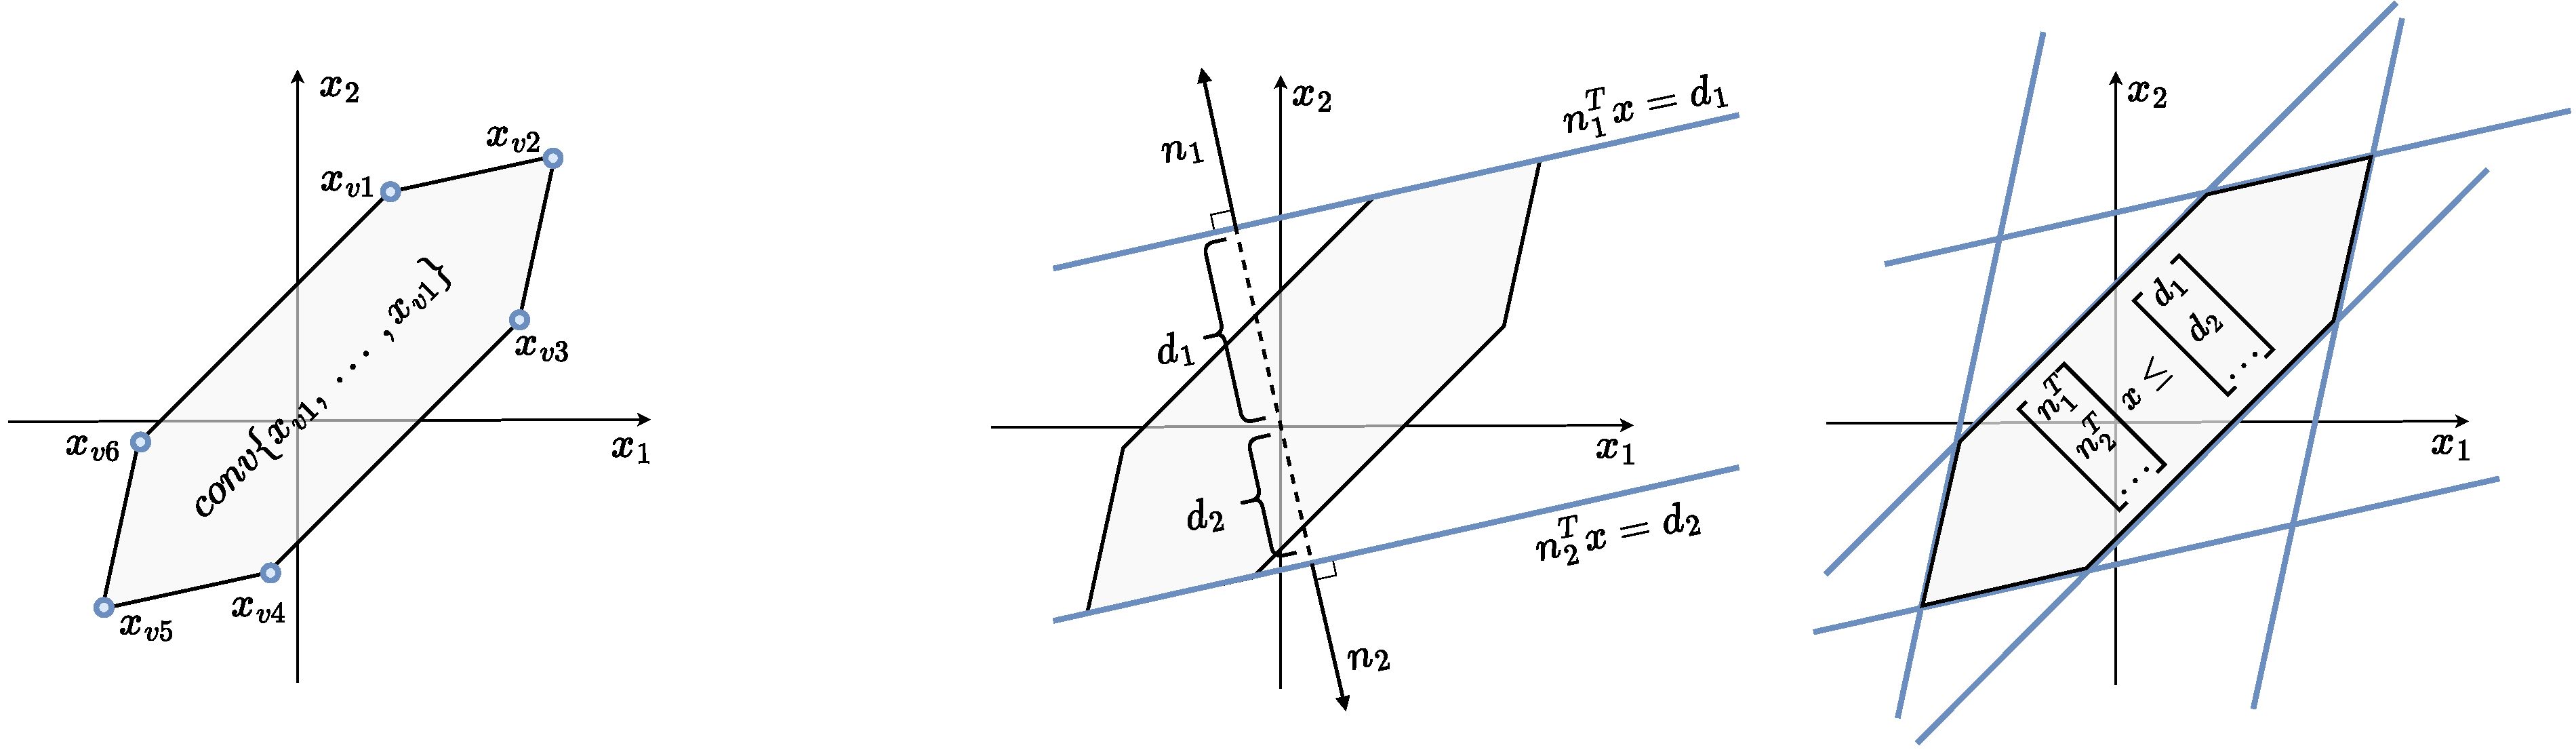
\includegraphics[width=\linewidth]{Chapters/imgs/h_v_rep.pdf}
    \caption{Caption}
    \label{fig:hv_rep}
\end{figure}

In the context of convex polytopes (denoted as $\mathcal{P}_x$) representing achievable task space variables $x\in\mathbb{R}^m$, the most commonly used representations in literature are so called vertex or $\repr{V}$ and half-plane or $\repr{H}$-representation \cite{henk2017basic, fukuda2004frequently}.  The algorithms that find the $\repr{V}$-representation of a polytope are often called \textit{vertex enumeration} algorithms, while the ones finding the $\repr{H}$-representation of are called \textit{facet enumeration} algorithms\cite{bremner_fukuda_marzetta_1998}. Figure \ref{fig:hv_rep} illustrates the difference between $\repr{V}$ and $\repr{H}$-representations using a two-dimensional polytope ($m = 2$). 

\paragraph*{Vertex of $\repr{V}$-representation}
This representation consist in specifying a list of polytope's vertices $\bm{x}_{vi}\in\mathbb{R}^m$, where the polytope is defined as their convex hull
\begin{equation}
\mathcal{P}_x = conv\{ \bm{x}_{v1},~\bm{x}_{v2},~ \ldots , ~\bm{x}_{vN} \}
\end{equation} 
Polytope $\repr{V}$-representation, in the case of physical ability metrics, is mostly used for visualisation purposes. The vertices $\bm{x}_{vi}\in\mathbb{R}^m$ can be easily transformed into triangulated meshes and visualised in standard visualisation tools, providing a visual insight into physical abilities of humans and robots. 

In the context of human-robot collaboration, an example application of polytope visualisation was proposed by Zolotas et al.\cite{Zolotas2021}, where the robot's velocity polytopes were used to inform the operator about the robot's movement capacity during the teleportation task.


\paragraph*{Half-plane or $\repr{H}$-representation}
This representation, on the other hand, is defined as the intersection of the half-planes forming the faces of the polytope
\begin{equation}
  \mathcal{P}_x = \{\bm{x} \in \mathbb{R}^m~ |~ H\bm{x} \leq \bm{d} \}
\end{equation} 
where the matrix $H \in \mathbb{R}^{N_f\times m }$ is composed of $N_f$ normal vectors $\bm{n}_i\in\mathbb
{R}^m$ of the half-planes corresponding to the $N_f$ faces of the polytope, while vector $\bm{d}\in \mathbb{R}^{N_f}$ contains their displacement $d_i$ from the origin. Figure \ref{fig:hv_rep} shows a graphical interpretation of the half-plane representation on a example of 2d ($m\!=\!2$) polytope. As with the $\repr{H}$-representation, the polytope can essentially be expressed as a set of convex linear constraints $H\bm{x}\leq\bm{d}$, it can be easily integrated in different optimisation problems, for example in robot control or trajectory planning applications. 

In the context of human-robot collaboration, being able to consider both robot's and human's physical abilities with in those contexts, opens doors for creating more human-centred robot control (or trajectory planning) strategies where robot's behaviour is adapted (planned), not just with respect to its own physical abilities, but also to the ones of the human.
Potential benefits of considering human's physical abilities for creating human-centred robot control were demonstrated in the context of assistive exoskeletons, for example in the work by Carmichael et al. \cite{carmichael_towards_2011} , where a coarse approximation of human's force was used, or by Petric et al.\cite{petric2019assistive}, where human's abilities were approximated using ellipsoids.

\paragraph*{} Furthermore, using standard polytope representations ($\repr{H}$ and $\repr{V}$) enables efficient use of standard polytope algorithms for evaluating different polytope algebra operations, such as Minkowski sums,  intersections or convex-hulls, providing an efficient way to compare and combine multiple polytopes. Several alternative polytope representations were proposed recently, such as $\repr{Z}$ \cite{kochdumper2019representation} and $\repr{M}$-representation \cite{sigl2023mrepresentation}, improving the efficiency of conducting polytope algebra operations, with respect to the traditional $\repr{H}$ and $\repr{V}$-representations. However, despite these advancements, their practical applications are still quite limited, primarily due to the challenging computational complexity involved in transforming polytopes into these alternative representations. 

In summary, when dealing with physical ability metrics based on polytopes, they are commonly expressed as a set of inequality and equality constraints. To efficiently work with these polytopes, it is necessary to convert them into a suitable representation such as $\repr{V}$ or $\repr{H}$. However, the choice of the polytope transformation algorithm, and its complexity, depends on various factors such as the polytope formulation (structure of its equality and inequality equations), the desired polytope representation ($\repr{V}$ or $\repr{H}$), and the time constraints for execution (whether online or offline). 

Therefore, following sections bring a classification of the polytope metrics with respect to their formulation, as well as an overview of the their applicable polytope transformation (vertex and facet enumeration) strategies.

% For example, the polytope of robot's achievable task space velocities from chapter \ref{ch:vel_poly}, where the robot has $n$ joints and task space is $m$ dimensional, can be expressed as
% \begin{equation}
%     \mathcal{P}_{v}(\bm{q}) = \{ \dot{\bm{x}} \in \mathbb{R}^m ~|~ \underbrace{A\dot{\bm{q}}\leq \bm{b}}_{\text{inequality}}, ~~ \underbrace{\dot{\bm{x}} = J(\bm{q})\dot{\bm{q}}}_{\text{equality}} \}
% \end{equation}
% where the equality equation $\dot{\bm{x}} = J(\bm{q})\dot{\bm{q}}$ corresponds to the robot's linearised kinematics through the state ${\bm{q}}\in\mathbb{R}^{n}$ dependant jacobian matrix $J(\bm{q}) \in \mathbb{R}^{m\times n}$, while the robot's joint velocity $\dot{\bm{q}}\in\mathbb{R}^{n}$ range  
% $\dot{\bm{q}}\in[\dot{\bm{q}}_{r,min},\dot{\bm{q}}_{r,max}]$ is expressed an inequality constraint $A\dot{\bm{q}}\leq\bm{b}$, using matrix $A\in\mathbb{R}^{2n\times n}$ and vector $\bm{b}\in \mathbb{R}^{2n}$.
% \begin{equation}
%     A= \begin{bmatrix}
%         I_{n\times n}\\
%         -I_{n\times n}
%     \end{bmatrix},\quad \bm{b} =\begin{bmatrix}
%         \dot{\bm{q}}_{r,max}\\
%         -\dot{\bm{q}}_{r,min}
%     \end{bmatrix}
% \end{equation}
% The equality and inequality equations defining the polytope $\mathcal{P}_v$ are expressed in the $n$ dimensional joint space of the robot, even though the polytope represents the limits of the task space variable $\dot{\bm{x}}\in\mathbb{R}^m$. Depending on the formulation and the number of inequality and equality equations of the polytope, different algorithms for polytope transformation are used to obtain a more standard and minimal representation of the polytope in the $m$ dimensional task space.

% Therefore, in order to be to compare or combine these metrics by applying different polytope algebra operations, such as Minkowski sum or intersection over these polytopes they first need to be transformed to a more suitable polytope representation. The same is true if these polytopes are to be visualised, then they need to be transformed to triangulated meshes. Finally, if the polytopes are to be used in different optimisation problems they need to be transformed to a set of linear inequality constraints over the $m$ dimensional output variable $\dot{\bm{x}}$.

\section{Generic view of polytope formulations}
\label{ch:generic_view}
% Polytope based physical ability metrics are often defined using a series of inequality equations, corresponding to the actuation limits, and the equality equations, corresponding to the linearised dynamics and kinematics equations. As an example, the polytope $\mathcal{P}_{v}$ of robot's achievable task space velocities $\dot{\bm{x}}\in\mathbb{R}^m$, from chapter \ref{ch:vel_poly}, is defined as
% \begin{equation}
%     \mathcal{P}_{v}(\bm{q}) = \{ \dot{\bm{x}} \in \mathbb{R}^m ~|~ \underbrace{\dot{\bm{q}}\in[\dot{\bm{q}}_{min},\dot{\bm{q}}_{max}]}_{\text{inequality}}, ~~ \underbrace{\dot{\bm{x}} = J(\bm{q})\dot{\bm{q}}}_{\text{equality}} \}
% \end{equation}
% where the equality equation $\dot{\bm{x}} = J(\bm{q})\dot{\bm{q}}$ corresponds to the robot's linearised kinematics through the jacobian matrix $J(\bm{q}) \in \mathbb{R}^{m\times n}$, while the robot's joint velocity range  
% $\dot{\bm{q}}\in[\dot{\bm{q}}_{min},\dot{\bm{q}}_{max}]$ can be expressed as an inequality constraint $A\dot{\bm{q}}\leq\bm{b}$, using matrix $A\in\mathbb{R}^{2n\times n}$ and vector $\bm{b}\in \mathbb{R}^{2n}$.
% \begin{equation}
%     A= \begin{bmatrix}
%         I_{n\times n}\\
%         -I_{n\times n}
%     \end{bmatrix},\quad \bm{b} =\begin{bmatrix}
%         \dot{\bm{q}}_{max}\\
%         -\dot{\bm{q}}_{min}
%     \end{bmatrix}
% \end{equation}

% Similar reasoning can be applied to most of the common physical ability metrics for robots and humans. However, with respect to the formulation of the inequality and equality equations of the polytopes their transformation to 

To effectively utilise polytopes of physical abilities in practical applications, it is necessary to transform them into standard representations such as $\repr{H}$ or $\repr{V}$-representation. While many algorithms have been proposed in the literature for manipulating polytope representations, they are often created for specific polytope formulations. Hence, this chapter aims to present a generic perspective on different families of polytope formulations commonly found when characterising the physical abilities of humans and robots. With the goal is to categorise these polytopes based on their formulation facilitating the choice of applicable algorithms.

From a generic standpoint, physical ability in a shape of polytope $\mathcal{P}_x$ can seen as feasible sets of output (task space) variables $\bm{x} \in \mathbb{R}^m$, produced by applying a linear transformation on the input (actuation space) variables $\bm{y} \in \mathbb{R}^n$, bounded within (actuator limits) a set $\bm{y}\in\mathcal{I}$. The input set $\mathcal{I}$, corresponding to the actuation limits, is often specified in a form of min-max intervals of the input variable $\bm{y}$
\begin{equation}
    \mathcal{I} = \{\bm{y}\in \mathbb{R}^n |~~ \bm{y}_{min} \leq \bm{y}\leq \bm{y}_{max} \}
    \label{eq:hypercube_lim}
\end{equation}
In a geometric sense, these individual intervals of the input variable $\bm{y}$ can be visualised as an $n$-dimensional hyperrectangle, also known as a hyperbox or an orthotope. Each axis $i$ of the hyperrectangle corresponds to an interval $y_i\in[y_{i,\text{min}},y_{i,\text{max}}]$.

In a general case, rather than interval, the input set $\mathcal{I}$ can be defined as any convex polytope (ex. set of linear constraints in its $\repr{H}$-representation).
\begin{equation}
    \mathcal{I} = \{\bm{y}\in \mathbb{R}^n|~~ H\bm{y}\leq \bm{d} \}
\end{equation}

Polytopes $\mathcal{P}_x$ are then defined as different linear transformations of the input set $\mathcal{I}$ (intervals or polytope shaped) from the $n$ dimensional input space to the $m$ dimensional output space, where input space is often higher dimensional $n>m$. In terms of their linear transformation formulation, physical abilities can be described with two main families of polytopes, namely the \textit{projection} and \textit{intersection} formulations.

\subsection{Projection formulation}
\label{ch:proj_formulaiton}
Projection formulation is defined through a linear affine transformation of the $n$ dimensional input space $\bm{y}\in\mathbb{R}^n$ to the $m$ dimensional output space $\bm{x}\in\mathbb{R}^m$ using the projection matrix $B\in \mathbb{R}^{m\times n}$
\begin{equation}
    \mathcal{P}_x=\{\bm{x}\in \mathbb{R}^m |~ \bm{x} = B\bm{y} + \bm{b}_x,~\bm{y} \in\mathcal{I} \}
    \label{eq:proj_poly}
\end{equation}
where $\bm{b}_x\in\mathbb{R}^m$ is a constant bias vector, defined in the output space. The name \textit{projection} formulation comes from the fact that the polytope $\mathcal{P}_x$ in this formulation is a projection of the $n$ dimensional input set $\mathcal{I}$ to the (usually lower) $m$ dimensional output space $\mathbb{R}^m$.

A graphical representation of the projection formulation (\ref{eq:proj_poly}) is shown on Figure \ref{fig:inter_proj}, where the input set $\mathcal{I}$ and the final polytope $\mathcal{P}_x$ are denoted in grey.


\subsection{Intersection formulation}
\label{ch:inter_formulaiton}
Intersection formulation, on the other hand, is expressed by a matrix equation $A\bm{x}=\bm{y}$, which can be interpreted as a linear transformation in the opposite direction\cite{LARSON2013}, from the $m$ dimensional input space $\bm{x}\in\mathbb{R}^m$ to the $n$ dimensional output space $\bm{y}\in\mathbb{R}^n$, using the projection matrix $A\in \mathbb{R}^{n\times m }$
\begin{equation}
    \mathcal{P}_x=\{\bm{x} \in \mathbb{R}^m|~ A\bm{x} = \bm{y}+ \bm{b}_y,~ \bm{y} \in \mathcal{I}\}
    \label{eq:inter_poly}
\end{equation}
where $\bm{b}_y \in \mathbb{R}^n$ is a constant bias vector, defined in the input space. The name \textit{intersection} formulation comes from the fact that the polytope $\mathcal{P}_x$ is no longer just a projection of the input set $\mathcal{I}$ to the $m$ dimensional output space, but rather a projection of its intersection with the image of the matrix $A$. 
A graphical representation of the intersection formulation (\ref{eq:inter_poly}) is shown on Figure \ref{fig:inter_proj}, where the intersection $\mathcal{I}\cap Im\{A\}$ and the final polytope $\mathcal{P}_x$ are denoted in blue.

The main difficulty of the intersection formulation (\ref{eq:inter_poly}) is that it is defined as an inverse projection, from the $m$ dimensional output space to the $n$ dimensional input space\cite{LARSON2013}. In order to inverse this relationship, an equivalent projection formulation polytope can be constructed by characterising the intersection $\mathcal{I}\cap Im\{A\}$. 

\begin{figure}
    \centering
    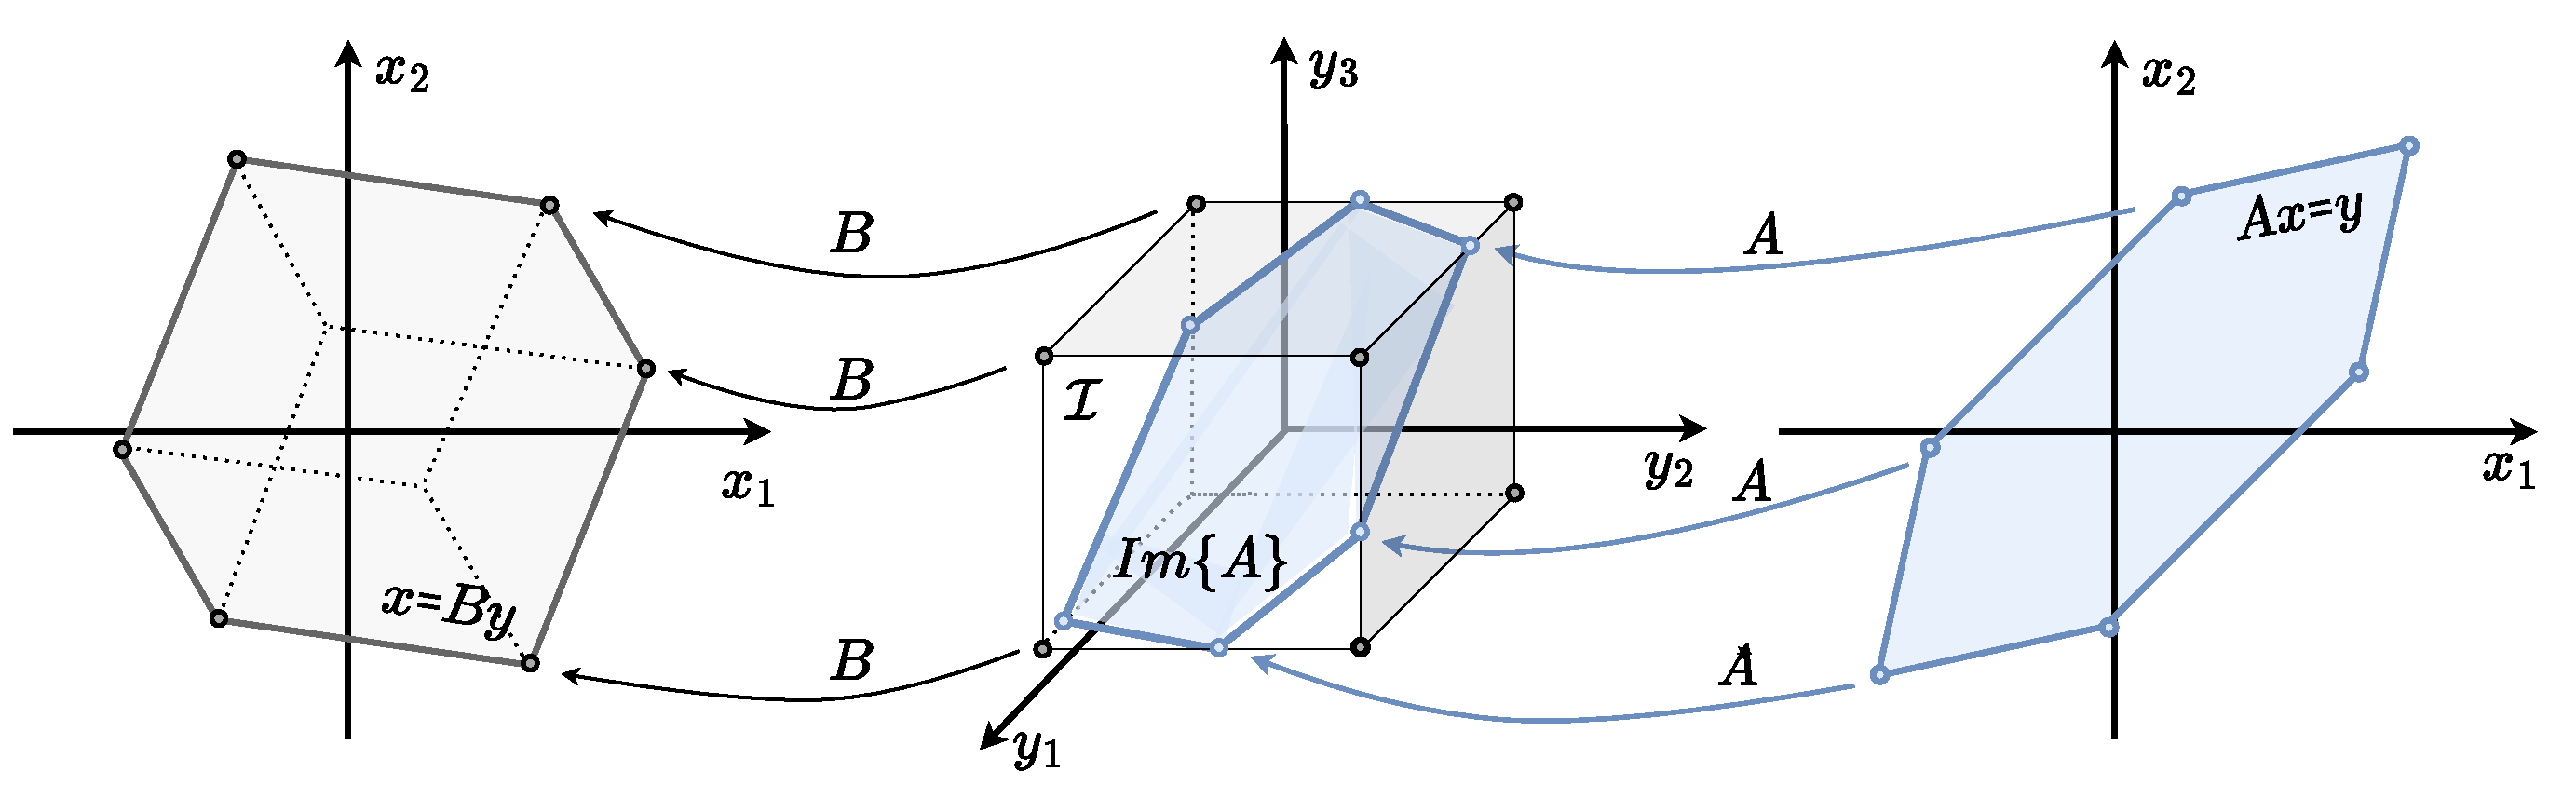
\includegraphics[width=\linewidth]{Chapters/imgs/intersection_projection.pdf}
    \caption{A comparative view of the projection (left) and intersection (right) polytope formulation using the same input space (middle). In the projection formulation, the whole input space $\mathcal{I}$ is projected using the matrix $B$ to the output space to obtain the polytope $\mathcal{P}_x$ (gray left). In the intersection formulation, first the intersection of the input space $\mathcal{I}$ with the image of the matrix $A$ has to be found (blue middle) $Im\{A\} \cap \mathcal{I}$ , then this intersection can be projected to the output space using the inverse of the matrix $A$ to obtain the polytope $\mathcal{P}_x$ (blue right).}
    \label{fig:inter_proj}
\end{figure}


\paragraph*{Equivalent projection formulation} 



%If bias $\bm{b}_y$ is neglected, the achievable set of the output variables $\mathcal{P}_x$, defined as in the matrix equation $A\bm{x}=\bm{y}$, will be entirely generated by the input variables $\bm{y}\in \mathbb{R}^n$, that can be described by the mapping $\bm{y} = A \bm{x}$. In other words, the input variables $\bm{y}$, described by this mapping, are a linear combination of $n$ column vectors $\bm{a}_i\in\mathbb{R}^n$ of the matrix $A$ \cite{LARSON2013}

If bias $\bm{b}_y$ is neglected, the input variables $\bm{y}$, described by this matrix equation $\bm{y} = A\bm{x}$, can be expressed as a linear combination of $n$ column vectors $\bm{a}_i\in\mathbb{R}^n$ of the matrix $A$ \cite{LARSON2013}
\begin{equation}
    \bm{y} = \bm{a}_1x_1 +  \bm{a}_2x_2 + \ldots +  \bm{a}_mx_m
\end{equation}
were $x_i$ are the $m$ components of output vector $\bm{x}$. This linear combination forms an $m$ dimensional subspace of the $n$ dimensional input space, spanned by $m$ column vectors $\bm{a}_i$, which is also called the image of the matrix $A$. 
\begin{equation}
    \bm{y}=A\bm{x} \in Im \{A\}
\end{equation}
The set of all the input variables $\bm{y}$ respecting the equation $\bm{y} = A \bm{x}$ and the limitations $\bm{y}\in\mathcal{I}$ can then be found as their intersection
\begin{equation}
   \bm{y} \in Im\{A\} \cap \mathcal{I}
    \label{eq:intersection_ai}
\end{equation}

Once the new input space defined by the intersection (\ref{eq:intersection_ai}) is found, an equivalent formulation of achievable output space polytope $\mathcal{P}_x$, can be found by projecting the intersection to the output space, typically using the inverse projection $\bm{x}=A^{-1}\bm{y}$. 
\begin{equation}
    \mathcal{P}_x = \{\bm{x}\in\mathbb{R}^m~|~\bm{x} = A^{-1} \bm{y}, \quad \bm{y} \in Im\{A\}\cap\mathcal{I}\}
\end{equation}
As in general case, the matrix $A$ is not invertible ($n>m$), the Moore-Penrose pseudo-inverse \cite{wang2018generalized} of the matrix $A^+ = A^T(AA^T)^{-1}$ can be used. Conveniently, as all the input variables $\bm{y}$, described by the equation (\ref{eq:intersection_ai}), belong to the image of the matrix $A$, the pseudo-inverse $A^+$ represents their unique inverse projector from the input to the output space
\begin{equation}
    \bm{x} = A^+ \bm{y}, ~\text{where} \quad \bm{y} \in Im\{A\}\cap\mathcal{I}
\end{equation}

Therefore,  by exploiting this relationship,  the equivalent formulation of the the initial intersection polytope formulation (\ref{eq:inter_poly}) can be expressed
\begin{equation}
\mathcal{P}_x=\{\bm{x}\in\mathbb{R}^m~|~ \bm{x} = A^+\bm{y},~ \bm{y} \in Im\{A\}\cap\mathcal{I}\} \label{eq:proj_inter}
\end{equation}
Figure \ref{fig:inter_proj} shows a graphical representation of this mapping where the intersection (\ref{eq:intersection_ai}) is shown in blue, as well as the final polytope $\mathcal{P}_x$ being its projection to the output space $\bm{x}\in \mathbb{R}^m$. 

If the bias vector $\bm{b}_y$ is not a zero vector the complete formulation becomes
\begin{equation}
\mathcal{P}_x=\{\bm{x} \in\mathbb{R}^m~|~ \bm{x} = A^+\bm{y} + A^+\bm{b}_y,~ \bm{y} + \bm{b}_y\in Im\{A\}\cap\mathcal{I}\} 
\end{equation}

Therefore, the intersection formulation (\ref{eq:inter_poly}) is generally more computationally complex to work with, than the projection formulation, as it requires characterising the intersection $Im\{A\}\cap\mathcal{I}$. 



\paragraph*{} The distinction between the intersection and projection formulation is important only if the matrices $A\in \mathbb{R}^{n\times m }$ and $B\in \mathbb{R}^{m\times n}$ do not have a full rank ($n\!>\!m$). If the matrices have full rank ($n\!=\!m$), the intersection formulation $A\bm{x} = \bm{y} + \bm{b}_y$ can be transformed to the projection formulation $\bm{x} = A^{-1}(\bm{y}+\bm{b}_y)$, as the matrix $A$ is square and invertible. In this case, the same strategies for transforming the polytope to an appropriate standard representation can be applied to both formulations.

In the case where the matrix $A$ does not have a full rank ($n\!>\!m$), as the matrix $A$ is no longer invertible, this manipulation is no longer possible, requiring different set of algorithms for its transformation. When characterising the physical abilities, as the polytopes map often higher dimensional input space (ex. joint space or muscle force space) to the lower dimensional output space (ex. 3D Cartesian space), the condition $n\!>\!m$ corresponds to the very common case where the redundant degrees of freedom are present. 

Figure \ref{fig:inter_proj} shows a geometric representation of the two polytope formulations on an example of a $n=3$ dimensional input space and $m=2$ dimensional output space, where the biases are set to zero vectors $\bm{b}_x=\bm{0}_2,\bm{b}_y=\bm{0}_3$.

\subsection{Special cases}
\label{ch:combined_forms}
Physical ability metrics described in chapter \ref{ch:poly_metrics} contain two special cases of polytope formulations that combine both intersection and projection formulations: \textit{intersection-projection} and \textit{projection-intersection} formulation.

\subsubsection{Intersection-projection formulation}
A special case polytope formulation, occurring with wrench and stiffness capacity of human musculoskeletal models, arises when the polytope has both intersection (\ref{eq:inter_poly}) and projection formulation (\ref{eq:proj_poly}). 
\begin{equation}
    \mathcal{P}_x \in \{\bm{x}\in \mathbb{R}^m~|~\underbrace{A \bm{x}= \bm{z}+ \bm{b}_z}_{\text{intersection}},~ \underbrace{ \bm{z}=B \bm{y}}_{\text{projection}} ,~ \bm{y} \in \mathcal{I}\} 
\end{equation}
where $\bm{x}\in\mathbb{R}^m$ is the output vector, $\bm{y} \in \mathbb{R}^d$ is an input vector and $\bm{z}\in\mathbb{R}^n$ is an intermediate space vector, where $d\!>\!n\!>\!m$. Matrix $B\in \mathbb{R}^{n \times d}$ is a projector matrix from $d$ dimensional input space to the $n$ dimensional intermediate space, matrix $A\in \mathbb{R}^{n\times m}$ is a projector matrix from $m$ dimensional output space to the $n$ dimensional intermediate space and $\bm{b}_z\in\mathbb{R}^n$ is the bias vector, defined in the intermediate space.

This formulations presents a special case of the intersection formulation with polytope shaped input set. It can also be expressed with
\begin{equation}
    \mathcal{P}_x \in \{\bm{x}\in \mathbb{R}^m~|~A \bm{x} = \bm{z} + \bm{b}_z,~ \bm{z} \in \mathcal{P}_z\} 
\end{equation}
where its input set polytope $\mathcal{P}_z$ is defined using the projection formulation
\begin{equation}
    \mathcal{P}_z \in \{\bm{z}\in \mathbb{R}^n~|~z = B\bm{y},~ \bm{y} \in \mathcal{I}\} 
\end{equation}

This formulation can also be transformed to an equivalent projection formulation using the same procedure as for the intersection formulation, resulting in a polytope 
\begin{equation}
\mathcal{P}_x=\{\bm{x} \in \mathbb{R}^m |~ \bm{x} = A^+\bm{z} - A^+\bm{b}_z,~ \bm{z}+\bm{b}_z \in Im{A}\cap\mathcal{P}_z\} 
\end{equation}

However, this polytope formulation is much more computationally complex than both intersection and projection formulation, as it requires first computing the projection polytope $\mathcal{P}_z$ and then finding the intersection $Im\{A\}\cap\mathcal{P}_z$ in order to find the polytope $\mathcal{P}_x$.


In case of wrench and stiffness capacity polytopes for human musculoskeletal models, the intermediate space is the space of joint torques $\bm{\tau}\in\mathbb{R}^n$, while the polytope $\mathcal{P}_z$ corresponds to the joint toque polytope $\mathcal{P}_{\bm{\tau}}$ from equation (\ref{eq:poly_torque_human}) constructed by the limits of human's muscle tensile forces $\bm{F}\in\mathbb{R}^d$.


\subsubsection{Projection-intersection formulation}
A special case polytope formulation, occurring with velocity capacity of human musculoskeletal models, arises when the polytope has both projection (\ref{eq:proj_poly}) and intersection formulation (\ref{eq:inter_poly}). 
\begin{equation}
    \mathcal{P}_x \in \{\bm{x}\in \mathbb{R}^m~|~ \underbrace{\bm{x} = B \bm{z} + \bm{b}_x}_{\text{projection}},~ \underbrace{A\bm{z}=\bm{y}}_{\text{intersection}},~ \bm{y} \in \mathcal{I}\} 
\end{equation}
where $\bm{x}\in\mathbb{R}^m$ is the output vector, $\bm{y} \in \mathbb{R}^d$ is an input vector and $\bm{z}\in\mathbb{R}^n$ is an intermediate space vector, where $d\!>\!n\!>\!m$. Matrix $A\in \mathbb{R}^{n \times d}$ is a projector matrix from $d$ dimensional input space to the $n$ dimensional intermediate space, matrix $B\in \mathbb{R}^{m\times n}$ is a projector matrix from $n$ dimensional intermediate space to the $m$ dimensional output space and $\bm{b}_x\in\mathbb{R}^m$ is the bias vector, defined in the output space.

Finally, this polytope formulation is a special case of a projection formulation with polytope shaped input set, and can be expressed as
\begin{equation}
    \mathcal{P}_x \in \{\bm{x}\in \mathbb{R}^m~|~ \bm{x} = B\bm{z} + \bm{b}_x,~ \bm{z} \in \mathcal{P}_z\} 
\end{equation}
where its input set polytope $\mathcal{P}_z$ is defined using the intersection formulation
\begin{equation}
    \mathcal{P}_z \in \{\bm{z}\in \mathbb{R}^n~|~Az = \bm{y},~ \bm{y} \in \mathcal{I}\} 
\end{equation}

This formulation can also be transformed to an equivalent projection formulation using the same procedure as for the intersection formulation, resulting in a polytope 
\begin{equation}
\mathcal{P}_x=\{\bm{x} \in \mathbb{R}^m |~ \bm{x} = BA^+\bm{y} + \bm{b}_x,~ \bm{y}\in Im\{A\}\cap\mathcal{I}\} 
\end{equation}

This polytope formulation is again much more computationally complex than both intersection and projection formulation, as it requires first computing the intersection $\bm{y} \in Im\{A\}\cap\mathcal{I}$, followed by the projection $BA^{+}\bm{y}$. 


In case of velocity capacity polytope for human musculoskeletal models, the intermediate space is the space of joint velocities $\dot{\bm{q}}\in\mathbb{R}^n$, while the polytope $\mathcal{P}_z$ corresponds to the joint toque polytope $\mathcal{P}_{\dot{\bm{q}}}$ from equation (\ref{eq:human_poly_joint_vel}) constructed by the limits of human's muscle extension velocities $\dot{\bm{l}}\in\mathbb{R}^d$.


\subsection{Categorising the polytope based metrics}
\label{ch:which_metric_which_formulation}

This chapter brings a classification of the common polytope based physical ability metrics for robotic systems, described in chapter \ref{ch:robot_metrics}, and for humans, described in chapter \ref{ch:human_metrics}, into four groups with respect to their formulation (projection or intersection) and input set $\mathcal{I}$ shape (interval or polytope). 

All the described polytope metrics can be classified within two formulations: intersection and projection formulation. 
Examples of the intersection formulation for robotic systems are wrench polytope \ref{ch:poly_force} and stiffness region polytope \ref{ch:robot_stiffness_poly}, where the matrix $A$ corresponds to the jacobian transpose matrix $J(\bm{q})^T$. For the human musculoskeletal models the same metrics, wrench polytope \ref{ch:force_poly_human} and stiffness region polytope \ref{ch:human_stiffness_poly}, are examples of intersection formulation, and again the matrix $A$ corresponds to their jacobian transpose matrices $J(\bm{q})^T$. All the other metrics, both for humans and robots belong to the projection formulation.

With respect to the input space limits $\mathcal{I}$, there are two classes of metrics: ones with interval limits (min-max ranges) and the others with polytope limits. All the robot metrics introduced in chapter \ref{ch:robot_metrics} have interval limits, while in the case of human musculoskeletal models the only one with interval limits is the acceleration polytope \ref{ch:human_aceleration_poly}. Wrench, velocity and stiffens region polytope based on musculoskeletal models have polytope shaped input space $\mathcal{I}$. Wrench and stiffness region polytope have input space $\bm{y}$ corresponding to the space of joint joint torques $\bm{\tau}$, which belonging to the polytope of achievable joint torques $\mathcal{P}_\tau$ (\ref{eq:poly_torque_human}). The velocity polytope has input space $\bm{y}$ corresponding to the space of joint velocities $\dot{\bm{q}}$ belonging to the joint velocity polytope $\mathcal{P}_{\dot{\bm{q}}}$ (\ref{eq:human_poly_joint_vel}).

Table \ref{tab:formulation_input_comparison} shows the list of the described polytope metrics with their corresponding formulations and input set $\mathcal{I}$ shapes.

% \begin{table}
% \centering
% \begin{tabular}{|l|c|c|c|c|c| c| c|}
% \hline
% Polytope Metric & $x$ & $A$ & $B$ & $y$ & $c$ & Dynamics & Collaboration \\
% \hline
%  \multicolumn{5}{c}{Robotic manipulators }  \\
% \hline
% Force/Wrench  & $\bm{f}$ & $J^T$ & - & $\bm{\tau}$ & $\bm{\tau}_b$ & Yes &$\oplus$ \\
% Velocity  & $\dot{\bm{x}}$ & - & $J$ & $\dot{\bm{q}}$ & - & No & $\cap$ \\
% Precision  & $\delta\dot{\bm{x}}$ & - & $J$ & $\delta\dot{\bm{q}}$ & - & No&  $\cap$ \\
% Acceleration  & $\ddot{\bm{x}}$ & - & $JM^{-1}$ & $\dot{\bm{\tau}}$ & $\bm{\tau}_b$ & Yes &   $\cap$ \\
% Jerk   & $\dddot{\bm{x}}$ & - & $J$ & $\dddot{\bm{q}}$ & $\bm{j}_b$ & No & $\cap$ \\
% Stiffness feasibility  & $\Delta\bm{x}$ & $J^T$ & - & $\bm{\tau}$ & $\bm{\tau}_b$ & Yes &$\oplus$ \\
% \hline
%  \multicolumn{5}{c}{Human musculoskeltal models}  \\
% \hline
% Force/Wrench & $\bm{f}$ & $J^T$ & $N$ & $\bm{F}$ & $\bm{\tau}_b$ & Yes &$\oplus$ \\
% Acceleration  & $\ddot{\bm{x}}$ & - & $JM^{-1}N$ & $\bm{F}$ & $\bm{\tau}_b$ & Yes &   $\cap$ \\
% Velocity  & $\dot{\bm{x}}$ & - & $J$ & $\dot{\bm{q}}$ & - & Yes &   $\cap$ \\
% Stiffness feasibility  &$\Delta\bm{x}$ & $J^T$ & $N$ & $\bm{F}$ & $\bm{\tau}_b$ & Yes &$\oplus$ \\
% \hline
% \end{tabular}
% \caption{Polytope bases physical ability metrics comparison}
% \label{tab:my_label}
% \end{table}


\begin{table}
\centering
\begin{tabular}{|l|c|c|c|c|c|}
\hline
Polytope Metric & Equation & $\bm{x}$ & Formulation &  $\bm{y}$ & Input set $\mathcal{I}$ \\
\hline
 \multicolumn{6}{c}{Robotic manipulators} \\
\hline
Velocity  & \ref{eq:poly_vel_rob}& $\dot{\bm{x}}$ & projection & $\dot{\bm{q}}$&$\dot{\bm{q}} \in [\dot{\bm{q}}_{min},\dot{\bm{q}}_{max}]$ \\
Kinematic Acceleration  & \ref{eq:poly_accel_kin} & $\ddot{\bm{x}}$  & projection & $\ddot{\bm{q}}$&$\ddot{\bm{q}}\in\ddot{\bm{q}}_{min},\ddot{\bm{q}}_{max}]$   \\
Kinematic Jerk  &\ref{eq:poly_jerk_kin} & $\dddot{\bm{x}}$ &  projection &$\dddot{\bm{q}}$&$\dddot{\bm{q}}\in[\dddot{\bm{q}}_{min},\dddot{\bm{q}}_{max}]$ \\
Precision  & \ref{eq:poly_precision_rob} & $\delta\dot{\bm{x}}$ & projection & $\delta{\bm{q}}$&$\delta{\bm{q}}\in[\delta{\bm{q}}_{min},\delta{\bm{q}}_{max}]$ \\
Force/Wrench &  \ref{eq:poly_force_rob} & $\bm{f}$ & intersection & $\bm{\tau}$&$\bm{\tau}\in [\bm{\tau}_{min},\bm{\tau}_{max}]$ \\
Acceleration  & \ref{eq:pol_accleration_rob} & $\ddot{\bm{x}}$ & projection & $\bm{\tau}$&$\bm{\tau}\in[\bm{\tau}_{min},\bm{\tau}_{max}]$ \\
Stiffness feasibility  &  \ref{eq:pol_sfr_rob}& $\Delta\bm{x}$ & intersection &$\bm{\tau}$&$\bm{\tau}\in[\bm{\tau}_{min},\bm{\tau}_{max}]$\\
\hline
 \multicolumn{6}{c}{Human musculoskeletal models} \\
\hline
Velocity &\ref{eq:velocity_polytope_human_ver_poly_lim}  & $\dot{\bm{x}}$ & projection & $\dot{\bm{q}}$&$\dot{\bm{q}}\in\mathcal{P}_{\dot{\bm{q}}}$ \\
% Force/Wrench & $\bm{f}$ & $J^T$ & $N$ & $[\bm{F}_{min},\bm{F}_{max}]$ & $\bm{F}$ & $\bm{\tau}_b$ \\
Force/Wrench & \ref{eq:human_force_poly_ver_poly_lim} &  $\bm{f}$ & intersection & $\bm{\tau}$&$\bm{\tau}\in\mathcal{P}_{\bm{\tau}}$ \\
Acceleration  & \ref{eq:poly_acceleration_hum} & $\ddot{\bm{x}}$ &projection & $\bm{F}$&$\bm{F}\in[\bm{F}_{min},\bm{F}_{max}]$  \\
% Stiffness feasibility  &$\Delta\bm{x}$ & $J^T$ & $N$ & $[\bm{F}_{min},\bm{F}_{max}]$ & $\bm{F}$ & $\bm{\tau}_b$ \\
Stiffness feasibility & \ref{eq:stiffness_human_all}  &$\Delta\bm{x}$  & intersection & $\bm{\tau}$&$\bm{\tau}\in\mathcal{P}_{\bm{\tau}}$ \\
\hline
\end{tabular}
\caption{Comparison of Polytope-based Physical Ability Metrics}
\label{tab:formulation_input_comparison}
\end{table}


\section{Polytope enumeration strategies} 
\label{ch:polytope_algorithms}

Transforming polytopes to their standard representations ($\repr{V}$ and $\repr{H}$) is well studied problem in literature. Over the years, many efficient algorithms have been proposed for vertex enumeration, finding $\repr{V}$-representation, and facet enumeration, finding $\repr{H}$-representation\cite{bremner_fukuda_marzetta_1998,fukuda_dd,avis_pivoting_nodate}. 

However, the algorithms are often developed for a specific polytope formulation, where their efficiency might vary considerably with the size of the problem (dimension of input and output spaces)\cite{avis_comparative_2015} and the complexity of the evaluated polytope (number of faces and vertices)\cite{Dyer1983}. Therefore, the choice of the appropriate polytope transformation algorithm depends on to the polytope formulation, the representation required by the application, as well as the required time-efficiency.

This chapter brings a non-exhaustive overview of standard algorithms for transforming different polytope formulations (intersection and projection) with different input set $\mathcal{I}$ shapes (interval and polytope) into different standard representations ($\repr{V}$ and $\repr{H}$). Additionally, chapter \ref{ch:approximation_algos} discusses different polytope approximation strategies in the context of improving the efficiency of the vertex and half-plane evaluation.

\subsection{Strategies for intersection formulation}
\label{ch:intersection_algos}

This chapter brings a short overview of methods used for transformation of polytopes with intersection formulation, described in chapter \ref{ch:inter_formulaiton}, into their respective $\repr{V}$ and $\repr{H}$-representation. First the simpler case of polytopes with the interval shaped input sets $\mathcal{I}$ are considered in chapter \ref{ch:inter_inter_chapter}, followed by the discussion of the steps necessary for transforming more generic polytopes with inputs set $\mathcal{I}$ having a polytope shape, in chapter \ref{ch:inter_poly_chapter}.

\subsubsection{Interval limits $\mathcal{I}$}
\label{ch:inter_inter_chapter}
\begin{figure}[!htb]
    \centering
    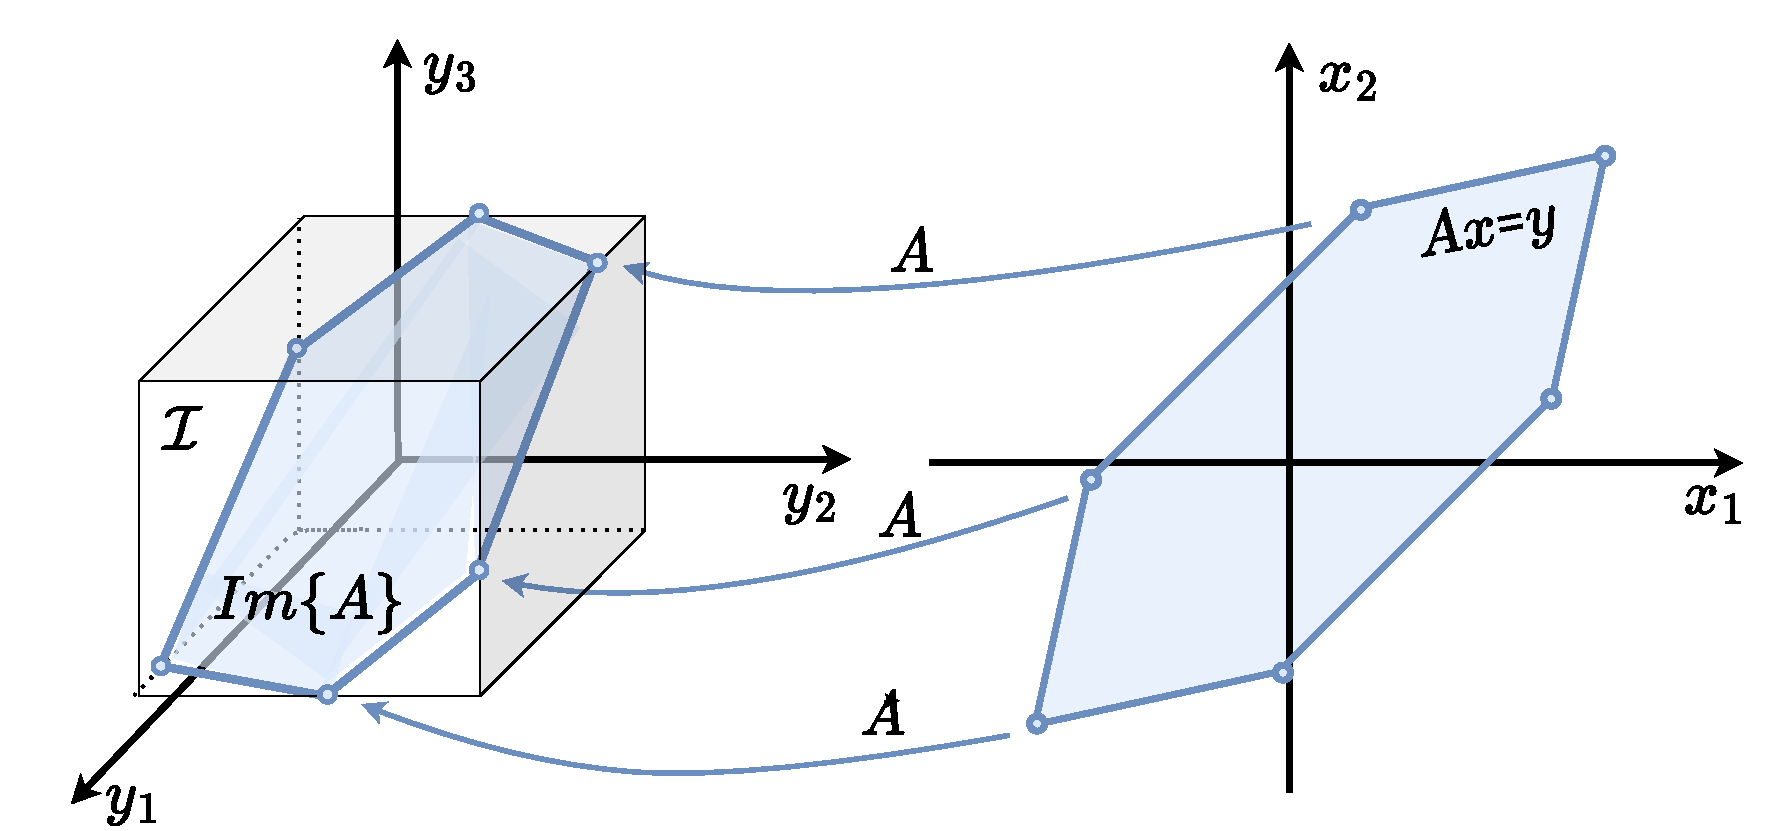
\includegraphics[width=0.7\linewidth]{Chapters/imgs/intersection.pdf}
    \caption{An example of the constructing an intersection formulation polytope with $m=2$ dimensional output space and $n=3$ dimensional input space. The intersection $Im\{A\} \cap \mathcal{I}$ of the hyperrectangle shaped input space $\mathcal{I}$ with the image of the matrix $A$ is shown in blue (left). This intersection can be projected to the output space using the inverse of the matrix $A$ to obtain the polytope $\mathcal{P}_x$ (blue right).}
    \label{fig:inter}
\end{figure}

The intersection polytope formulation (\ref{eq:inter_poly}) with the interval limits (\ref{eq:hypercube_lim}) is a spacial case of the intersection polytope formulation where the input space limits $\mathcal{I}$ are defined as independent min-max ranges 

\begin{equation}
    \mathcal{P}_x=\{\bm{x}\in\mathbb{R}^m |~ A\bm{x} = \bm{y},~\bm{y}_{min} \leq  \bm{y} \leq \bm{y}_{max}  \}
    \label{eq:inter_hyp}
\end{equation}
where $\bm{y}\in\mathbb{R}^n$ is an $n$ dimensional input vector, $\bm{x}\in\mathbb{R}^m$ is the $m$ dimensional output vector and $A\in\mathbb{R}^{n\times n}$ is a transformation matrix from output to the input space.

The geometrical representation of the polytope $\mathcal{P}_x$ defined by (\ref{eq:inter_hyp}) is shown on Figure \ref{fig:inter}, for the example of $n=3$ dimensional interval $\mathcal{I}$ and $m=2$ dimensional polytope $\mathcal{P}_x$. 
The resulting polytope $\mathcal{P}_x$ is an affine projection of the intersection of the hyperrectangle (interval) $\mathcal{I}$ and the image of the matrix $A$ ($Im\{A\}$) into the lower dimensional output space. As shown on Figure \ref{fig:inter}, the vertices and faces of the polytope $\mathcal{P}_x$ do not correspond to the projection of the vertices and faces of the hyperrectangle (interval) $\mathcal{I}$. 
Rather, as show in equation (\ref{eq:proj_inter}), the polytope $\mathcal{P}_x$ is generated by projecting the intersection $Im\{A\}\cap\mathcal{I}$, of the hyperrectangle (interval) $\mathcal{I}$ and the image of the matrix $A$, to the output space. 
Therefore, there is a unique mapping between the vertices and faces of the intersection $Im\{A\}\cap\mathcal{I}$, and the vertices and the faces of the polytope $\mathcal{P}_x$, given through the Moore-Penrose inverse\cite{wang2018generalized} of the matrix $A$. 

\paragraph*{$\repr{H}$-representation} Finding the $\repr{H}$-representation of such polytope can be done directly by substituting $\bm{y}$ with $A\bm{x}$ in the interval equation $\bm{y}\in[\bm{y}_{min},\bm{y}_{max}]$ and rewriting it in the matrix from
\begin{equation}
   \underbrace{\begin{bmatrix}
        A\\
        -A
    \end{bmatrix}}_{H}\bm{x} \leq \underbrace{\begin{bmatrix}
         \bm{y}_{max}\\
        -\bm{y}_{min} 
    \end{bmatrix} }_{\bm{d}}
\end{equation}
where matrix $H\in\mathbb{R}^{2n \times m}$ and the vector $\bm{d}\in\mathbb{R}^{2n}$ can be used to express the $\repr{H}$-representation of the polytope $\mathcal{P}_x$
\begin{equation}
    \mathcal{P}_x=\{\bm{x}\in\mathbb{R}^m |~ H\bm{x} \leq \bm{d} \}
    \label{eq:inter_h_rep}
\end{equation}
 Even though this $\repr{H}$-representation (\ref{eq:inter_h_rep}) of the polytope $\mathcal{P}_x$ follows directly from its definition and can be easily expressed, it might not be minimal. This means that even though the equation (\ref{eq:inter_h_rep}) is correct and fully describes the polytope $\mathcal{P}_x$, there might be some redundant half-plane constraints $n_i^T\bm{x}\leq d_i$. Many algorithms have been developed over the years for removing the redundant constraints $H\bm{x}\leq\bm{d}$ \cite{Paulraj2006}, and their computational complexity is generally equivalent to solving a series of linear programming (LP) problems \cite{Telgen1983}. Therefore, depending on the application and the computational complexity of the polytope description necessary, such techniques can be used to reduce the equation (\ref{eq:inter_h_rep}) to the minimal set of linear constraints $H\bm{x}\leq \bm{d}$.
 
\paragraph*{$\repr{V}$-representation} 
When it comes vertex enumeration of polytopes many algorithms have been developed in the literature, where some of the most important ones are based on Double Description Method (DDM)\cite{fukuda_dd} or different versions of a Pivoting Methods (PIM)\cite{avis_pivoting_nodate} both introduced by Fukuda and Avis. They both formulate the vertex enumeration problem as transformation of a half-plane representation to a vertex representation, and they both can be used in both directions, from $\repr{H}$ to $\repr{V}$, as well as from $\repr{V}$ to $\repr{H}$. 

When it comes to the intersection formulation polytope with interval input set $\mathcal{I}$, these methods can be used very efficiently by leveraging the fact that the half-plane representation (\ref{eq:inter_h_rep}) can be easily obtained. These generic algorithms are well suited and relatively efficient for different high and low dimensional problems \cite{avis_comparative_2015}. However, when it comes to computational efficiency, methods that show the best results are often the ones leveraging the specific geometry of their problems. 

An efficient algorithm for vertex enumeration of the intersection type polytope has been proposed by Gouttefarde et al. \cite{gouttefarde_versatile_2015} for the use-case in the redundancy resolution of the cable driven parallel robots, where the the matrix $A$ is the cable null-space projector of the wrench matrix $N=null\{W\}$, input vector $\bm{y}$ is the vector of cable tensions $\bm{t}\in\mathbb{R}^n$ and the output vector $\bm{x}$ corresponds to the null-space vector $\bm{\lambda}\in\mathbb{R}^m$. This algorithm exploits the geometry of the problem assuming that the wrench matrix null-space is always $m=2$ dimensional, in which case the polytope becomes a 2D polygon, which boundaries are then efficiently navigated in search for extremities. However, this algorithm does not scale well to higher dimensional problems.

In the case of the robotic manipulator's wrench polytope, described in chapter \ref{ch:poly_force} and which has the intersection formulation as well, where the matrix $A$ is the jacobian transpose matrix $J^T$, the input vector $\bm{y}$ is the vector of joint torques $\bm{\tau}\in\mathbb{R}^n$ and the output vector $\bm{x}$ is a vector of cartesian wrenches $\bm{f}\in\mathbb{R}^m$. For this problem, Chiacchio et al. \cite{chiacchio_evaluation_1996} have proposed an algorithm for finding its vertices that performs an exhaustive search through the input hyperrectangle (interval) limits $\mathcal{I}$. This algorithm has been improved by Sasaki et al. \cite{sasaki_vertex_nodate} where the computational complexity has been significantly reduced by exploiting the geometry of the intersection of the hyperrectangle (interval) $\mathcal{I}$ and the image of matrix $Im\{A\}$, leveraging the polytope formulation (\ref{eq:proj_inter})
\begin{equation}
\mathcal{P}_x=\{\bm{x}\in\mathbb{R}^m |~ \bm{x} = A^+\bm{y},~ \bm{y} \in Im\{A\}\cap[\bm{y}_{min},\bm{y}_{max}]\}
\label{eq:inter_hyp_inter}
\end{equation}


\paragraph*{}In the absence of the exact method for finding the polytope's $\repr{H}$ or $\repr{V}$-representation with an acceptable execution time for the given application, polytope approximation strategies described in Chapter \ref{ch:approximation_algos} may present a viable solution. 

\subsubsection{Polytope limits $\mathcal{I}$}
\label{ch:inter_poly_chapter}
\begin{figure}[h]
    \centering
    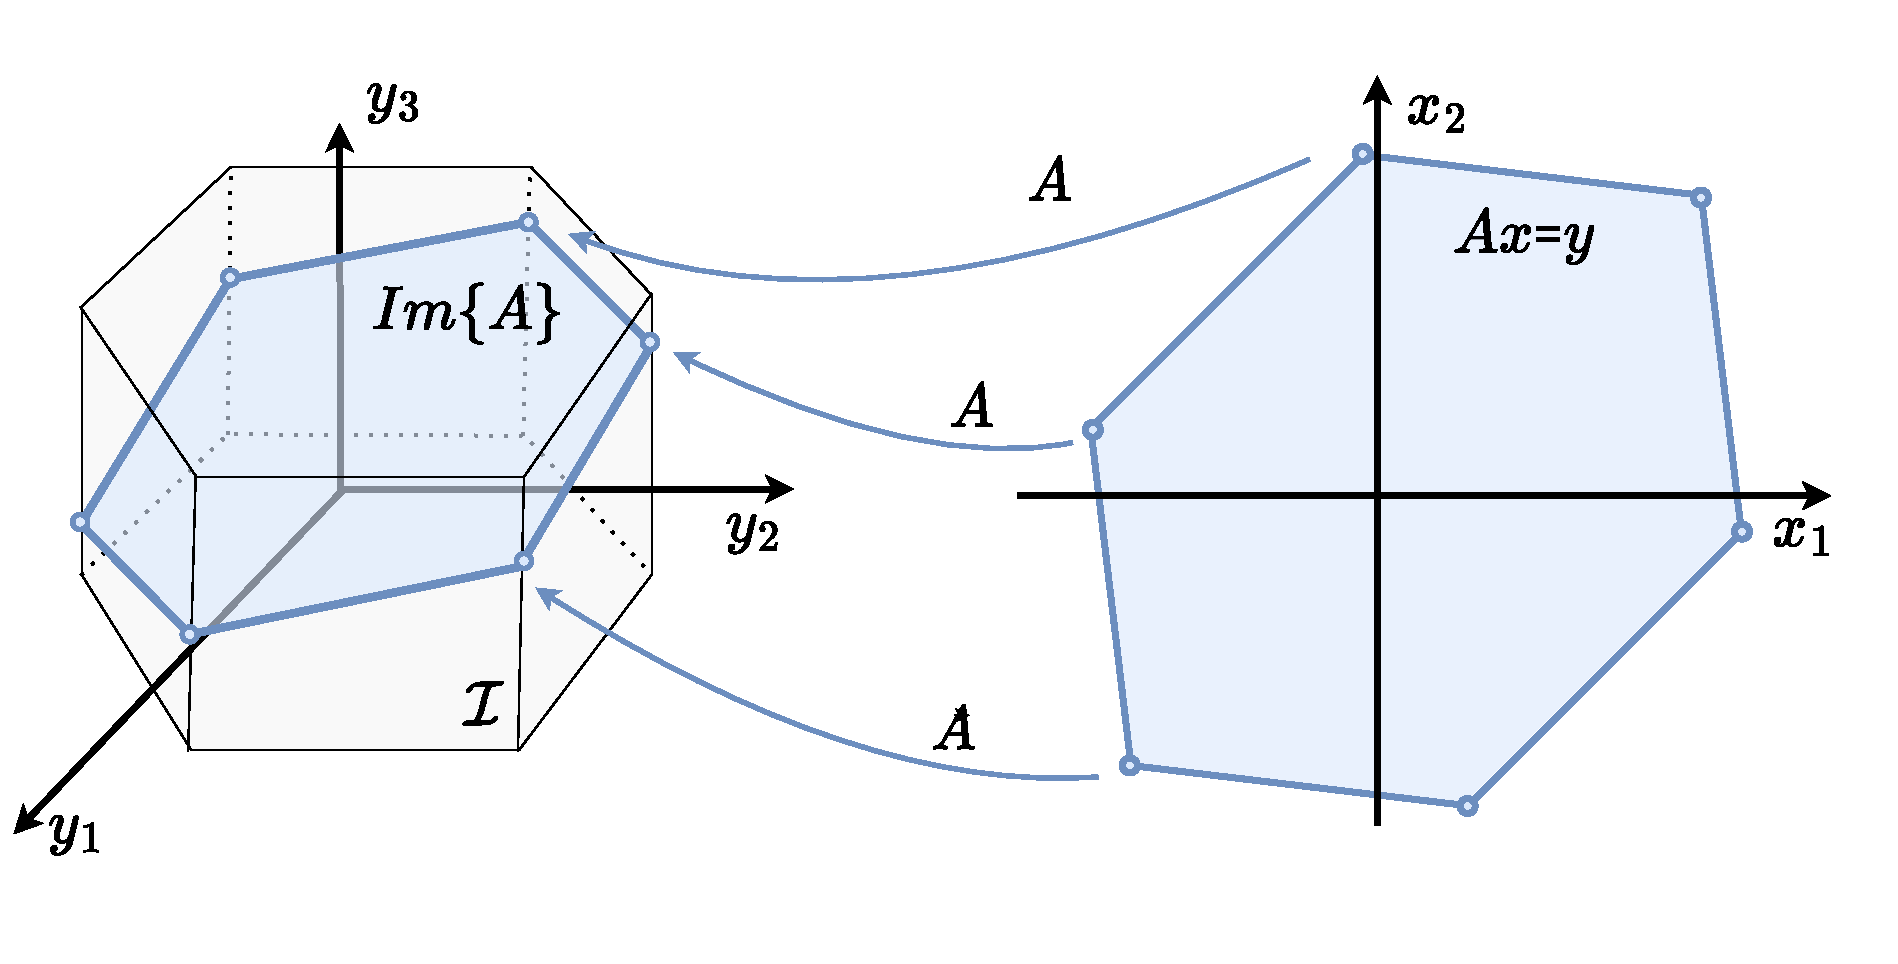
\includegraphics[width=0.7\linewidth]{Chapters/imgs/inter_poly.pdf}
    \caption{An example of the constructing an intersection formulation polytope with $m=2$ dimensional output space and $n=3$ dimensional input space. The input set $\mathcal{I}$ has a polytope form, and its intersection with the image of the matrix $A$ is shown in blue (left). The final polytope $\mathcal{P}_x$ is shown in blue as well (right).}
    \label{fig:inter_poly}
\end{figure}



This intersection polytope (\ref{eq:inter_poly}) with polytope input set $\mathcal{I}$ can be expressed as
\begin{equation}
    \mathcal{P}_x=\{\bm{x}\in\mathbb{R}^m |~ A\bm{x} = \bm{y},~\bm{y} \in \mathcal{I}  \}
\end{equation}
where $\bm{y}\in\mathbb{R}^n$ is an $n$ dimensional input vector, $\bm{x}\in\mathbb{R}^m$ is the $m$ dimensional output vector and $A\in\mathbb{R}^{n\times n}$ is a transformation matrix from output to the input space.

When the input space $\mathcal{I}$ has a polytope shape, given its structure, finding the $\repr{V}$ or $\repr{H}$-representation of this intersection polytope $\mathcal{P}_x$ varies in difficulty. 
The geometrical interpretation of the intersection remains very similar as in the case of the hyperrectangle (interval) $\mathcal{I}$, however this time the image of the matrix $A$ is intersected with the polytope $\mathcal{I}$, as shown in a example on Figure \ref{fig:inter_poly}.

\paragraph*{$\mathcal{I}$ expressed with $\repr{H}$-representation } When the polytope $\mathcal{I}$ is expressed by its $\repr{H}$-representation 
\begin{equation}
    \mathcal{I} = \{ \bm{y}\in \mathbb{R}^n ~|~H\bm{y} \leq \bm{d}\}
\end{equation}
then finding the $\repr{H}$-representation of the polytope $\mathcal{P}_x$ is straightforward, by replacing the vector $\bm{y}$ with $A\bm{x}$
\begin{equation}
    \mathcal{P}_x=\{\bm{x}\in  \mathbb{R}^m|~ HA\bm{x} \leq \bm{d} \}
    \label{eq:inter_poly_h_rep}
\end{equation}
Even though this formulation fully determines the polytope $\mathcal{P}_x$ it might contain some redundant half-plane equations, therefore if the application requires it, different algorithms for removal of redundant inequalities can be used \cite{Paulraj2006}.

Finding the $\repr{V}$-representation of the polytope $\mathcal{P}_x$, given the $\repr{H}$-representation  of the input polytope $\mathcal{I}$, can then be performed by first expressing the polytope $\mathcal{P}_x$ in its $\repr{H}$-representation (\ref{eq:inter_poly_h_rep}), followed by applying standard vertex enumeration methods such as DDM\cite{fukuda_dd} or PIM\cite{avis_pivoting_nodate} based methods. 



\paragraph*{$\mathcal{I}$ expressed with $\repr{V}$-representation } 
In the case where the polytope $\mathcal{I}$ is expressed by its $\repr{V}$-representation, 
\begin{equation}
    \mathcal{I} = conv\{ \bm{y}_{v1}, ~ \bm{y}_{v2},~ \ldots\}
\end{equation}
these vertices can be transformed to the $\repr{H}$-representation using techniques such as DDM \cite{fukuda_dd} or different convex-hull algorithms \cite{Barber1996}, which can then be used with the above described approach.

\paragraph*{$\mathcal{I}$ expressed differently} Polytope $\mathcal{I}$, in general case, can have different formulation that does not correspond to neither $\repr{V}$ or $\repr{H}$-representation. For example, as discussed in chapter \ref{ch:combined_forms}, the wrench and stiffness capacity of human musculoskeletal models have intersection form with polytope limits, while the input polytope has a projection (\ref{eq:proj_poly}) formulation. But more generally, it could have an intersection formulation (\ref{eq:inter_poly}) itself or might include additional equality and inequality constraints. 

In those cases the same approach can be applied to $\mathcal{I}$, first it can be transformed to the $\repr{H}$-representation, which can then be directly used to find the $\repr{H}$ or $\repr{V}$-representation of the polytope $\mathcal{P}_x$, as described above.

\paragraph*{} In cases where the time-efficiency of finding the $\repr{H}$ representation of the polytope $\mathcal{I}$ or even enumerating vertices of the polytope (\ref{eq:inter_poly_h_rep}) might be not appropriate for given application, polytope approximation strategies described in Chapter \ref{ch:approximation_algos} might be a viable option.

\subsection{Strategies for projection formulation}
\label{ch:projection_algos}

This chapter brings a short overview of methods used for transformation of polytopes with projection formulation, described in chapter \ref{ch:proj_formulaiton}, into their respective $\repr{V}$ and $\repr{H}$-representation. First the simpler case of polytopes with the interval shaped input sets $\mathcal{I}$ are considered in chapter \ref{ch:proj_inter_chapter}, followed by the discussion of the steps necessary for transforming more generic polytopes with inputs set $\mathcal{I}$ having a polytope shape, in chapter \ref{ch:proj_poly_chapter}.

\subsubsection{Interval limits $\mathcal{I}$}
\label{ch:proj_inter_chapter}
\begin{figure}[!htb]
    \centering
    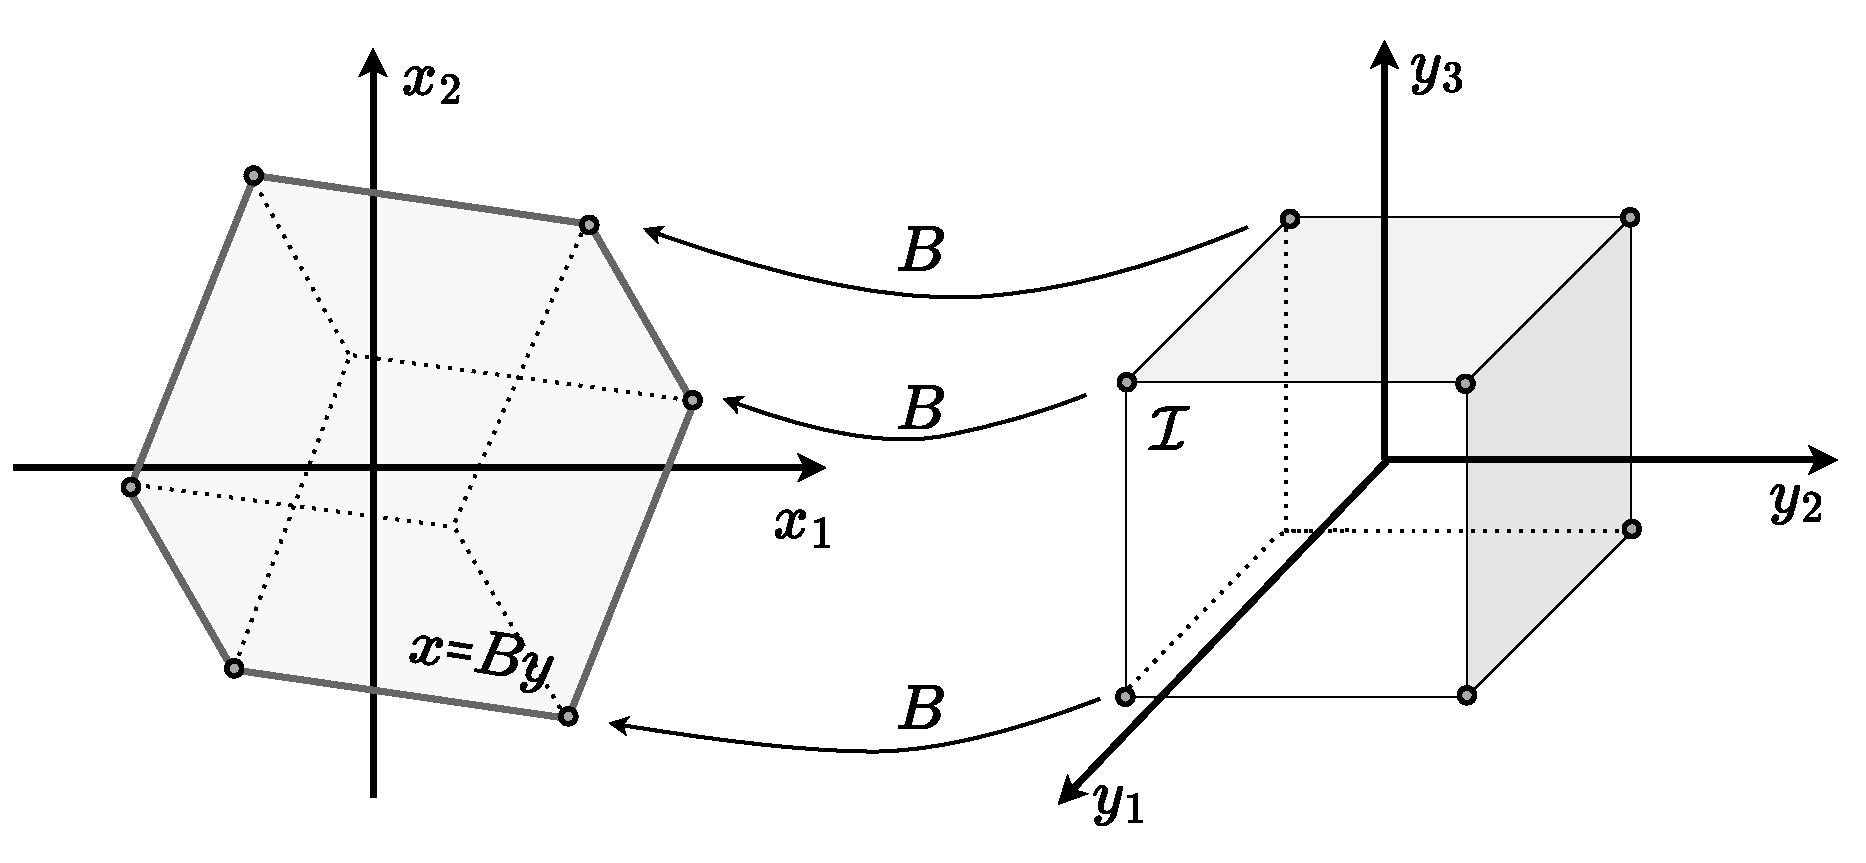
\includegraphics[width=0.7\linewidth]{Chapters/imgs/projection.pdf}
    \caption{An example of the constructing a projection formulation polytope with $m=2$ dimensional output space and $n=3$ dimensional input space, where the input space $\mathcal{I}$ has a hyperrectangle shape. In the projection formulation, the whole input space $\mathcal{I}$ is projected using the matrix $B$ to the output space to obtain the polytope $\mathcal{P}_x$ (gray left). }
    \label{fig:proj}
\end{figure}

The projection polytope formulation (\ref{eq:proj_poly}) with the interval limits (\ref{eq:hypercube_lim}) is a spacial case of the projection polytope where the input space limits $\mathcal{I}$ are defined as independent min-max ranges 
\begin{equation}
    \mathcal{P}_x=\{\bm{x} \in \mathbb{R}^m|~ \bm{x} = B\bm{y},~\bm{y}_{min} \leq  \bm{y} \leq \bm{y}_{max}  \}
    \label{eq:proj_hyp}
\end{equation}
where $\bm{y}\in\mathbb{R}^n$ is an $n$ dimensional input vector, $\bm{x}\in\mathbb{R}^m$ is the $m$ dimensional output vector and $B\in\mathbb{R}^{m\times n}$ is a transformation matrix from input to the ouptut space.

The geometrical representation of the polytope $\mathcal{P}_x$ defined by (\ref{eq:proj_hyp}) is shown on Figure \ref{fig:proj}, for the example of $n=3$ dimensional hyperrectangle (interval) $\mathcal{I}$ and $m=2$ dimensional polytope $\mathcal{P}_x$. The resulting polytope $\mathcal{P}_x$ is an affine projection of the hyperrectangle (interval)$\mathcal{I}$ into the lower dimensional output space. And all the vertices and the faces of the polytope $\mathcal{P}_x$ correspond directly to the projection of the vertices and faces of the hyperrectangle (interval) $\mathcal{I}$. 
 
\paragraph*{$\repr{V}$-representation} The most straight-forward way of finding the vertices $\bm{x}_{vi}\in\mathbb{R}^m$ of the projection polytope $\mathcal{P}_x$ is by first enumerating the $2^n$ vertices $\bm{y}_{vi}\in\mathbb{R}^n$ of the hyperrectangle  (interval) $\mathcal{I}$, by creating a list of all the combinations of the minimal $\bm{y}_{min}$ and maximal $\bm{y}_{max}$ values of $\bm{y}$
\begin{equation}
    \bm{y}_{v1} = \begin{bmatrix}
        y_{1,min}\\
        y_{2,min}\\
        \ldots\\
        y_{n,min}\\
    \end{bmatrix},\quad
    \bm{y}_{v2} = \begin{bmatrix}
        y_{1,max}\\
        y_{2,min}\\
        \ldots\\
        y_{n,min}\\
    \end{bmatrix},\qquad\ldots,\qquad
    \bm{y}_{v2^n} = \begin{bmatrix}
        y_{1,max}\\
        y_{2,max}\\
        \ldots\\
        y_{n,max}\\
    \end{bmatrix} 
\end{equation}
Then these vertices can be projected to the lower dimensional output space $\mathbb{R}^m$ using the projection matrix $B\in \mathbb{R}^{m\times n}$, where the polytope $\mathcal{P}_x$ can be found by calculating their convex-hull of the projected points.
\begin{equation}
    \mathcal{P}_x = conv\{B\bm{y}_{v1},B\bm{y}_{v2},~\ldots, ~ B\bm{y}_{v2^n}\}
\end{equation}

The complexity of this approach depends on two factors. The dimension of the of the input space $\bm{y} \in \mathbb{R}^n$ and the dimension of the output space $\bm{x}\in \mathbb{R}^m$. The number of vertices of the hyperrectangle (interval) is grows exponentially $2^n$ with the dimension of the input space $n$, and constructing a matrix of $2^n \times n$ entries can become impractical. On the other hand, as this approach requires a convex-hull algorithm to be run in the $m$-dimensional output space, the dimension $m$ might make the convex-hull algorithm impractical as their complexity grows significantly with the dimension of the space $m$ \cite{Barber1996}.

Therefore for higher dimensional input and output spaces it might be more efficient to first calculate the $\repr{H}$-representation  of this polytope, using the methods described in the following section, and then use a vertex enumeration methods, such as DDM\cite{fukuda_dd} or PIM\cite{avis_pivoting_nodate}, to find the $\repr{V}$-representation.

\paragraph*{$\repr{H}$-representation} A naive approach to finding the $\repr{H}$-representation of the projection formulation (\ref{eq:proj_hyp}) is to decouple the problem and first find the vertex representation of the polytope $\mathcal{P}_x$ and then use the standard vertex enumeration algorithms, such as DDM \cite{fukuda_dd} or PIM\cite{avis_pivoting_nodate}, to find the $\repr{H}$-representation.

However, there are several more efficient algorithms in the literature finding the half-plane representation of the projection formulation (\ref{eq:proj_hyp}) directly. One of the most well known algorithms for this specific case is arguably Fourier-Motzkin elimination (FME), described by Dantzig and Eaves \cite{dantzig1973fourier}. This algorithm uses an iterative inequality elimination method to isolate the set of half-plane equations bounding the polytope $\mathcal{P}_x$. However, this approach has a significant complexity and does not guarantee minimal representation \cite{Monniaux2010}. 
A more efficient algorithm was introduced Bouchard et al. \cite{Bouchard2009} and improved by Gouttefarde and Krut \cite{hyper_psm}, called Hyper-Plane Shifting Method (HPSM). This algorithm finds the minimal $\repr{H}$-representation of the polytope (\ref{eq:proj_hyp}) by efficiently performing the exhaustive search of all the possible half-plane combinations. Even-though much more efficient than the Fourier-Motzkin elimination, as it relies on the exhaustive search, it has exponential complexity with the dimension $n$ of the input interval $\mathcal{I}$.

\paragraph*{}Like in the case of the intersection formulation, when the exact methods do not satisfy the time efficiency of a given application, polytope approximation strategies described in Chapter \ref{ch:approximation_algos} may present a viable solution. 


\subsubsection{Polytope limits $\mathcal{I}$}
\label{ch:proj_poly_chapter}
\begin{figure}[h]
    \centering
    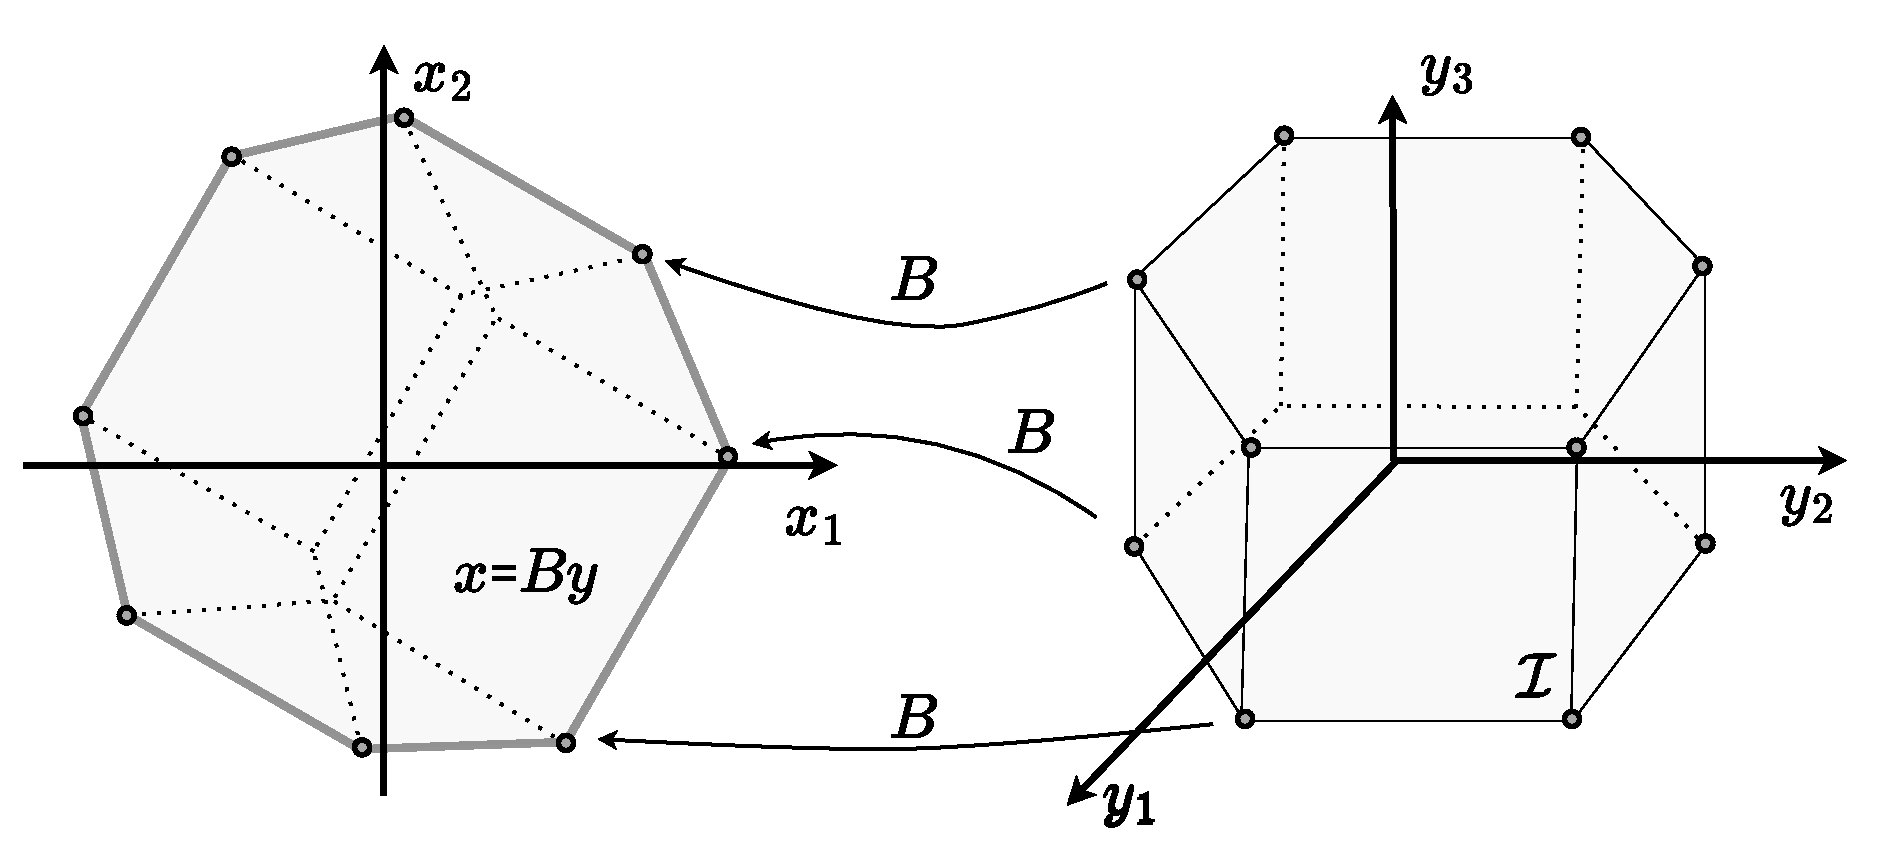
\includegraphics[width=0.7\linewidth]{Chapters/imgs/proj_poly.pdf}
    \caption{An example of the constructing a projection formulation polytope with $m=2$ dimensional output space and $n=3$ dimensional input space, where the input space $\mathcal{I}$ has a polytope shape. In this formulation, the whole input space $\mathcal{I}$ is projected using the matrix $B$ to the output space to obtain the polytope $\mathcal{P}_x$ (gray left). }
    \label{fig:proj_poly}
\end{figure}

The projection polytope (\ref{eq:proj_poly}) with polytope input set $\mathcal{I}$ can be expressed as
\begin{equation}
    \mathcal{P}_x=\{\bm{x}\in\mathbb{R}^m |~ \bm{x} = B\bm{y},~\bm{y} \in \mathcal{I}  \}
    \label{eq:proj_poly_1}
\end{equation}
where $\bm{y}\in\mathbb{R}^n$ is an $n$ dimensional input vector, $\bm{x}\in\mathbb{R}^m$ is the $m$ dimensional output vector and $B\in\mathbb{R}^{n\times m}$ is a transformation matrix from input to the output space.
When the input limits $\mathcal{I}$ have a form of a polytope, depending on the way $\mathcal{I}$ is defined, there are different ways to find projection polytope (\ref{eq:proj_poly_1}) vertex and half-plane representation. 

The geometrical representation of the polytope $\mathcal{P}_x$ defined by (\ref{eq:proj_poly_1}) is shown on Figure \ref{fig:proj_poly}, for the example of $n=3$ dimensional polytope $\mathcal{I}$ and $m=2$ dimensional polytope $\mathcal{P}_x$. The resulting polytope $\mathcal{P}_x$ is an affine projection of the polytope $\mathcal{I}$ into the lower dimensional output space. Furthermore, the vertices and the faces of the polytope $\mathcal{P}_x$ correspond to the subset of the projected vertices and faces of the polytope $\mathcal{I}$. 


\paragraph*{$\mathcal{I}$ expressed with $\repr{V}$-representation } If polytope $\mathcal{I}$ is expressed using its vertex or $\repr{V}$-representation
\begin{equation}
    \mathcal{I} = conv\{ \bm{y}_{v1}, ~ \bm{y}_{v2},~ \ldots\}
\end{equation}
where $\bm{y}_{vi}\in\mathbb{R}^n$ are the vertices of the polytope $\mathcal{I}$, the projection formulation polytope (\ref{eq:proj_poly_1}) can be found by projecting the vertices of $\mathcal{I}$ to the output space using the matrix $B \in \mathbb{R}^{m\times n}$ and calculating the convex-hull of the projected vertices
\begin{equation}
    \mathcal{P}_x= conv\{ B\bm{y}_{v1}, ~ B\bm{y}_{v2},~ \ldots\}
\end{equation}
The convex-hull algorithm finds the $\repr{V}$-representation of the projection polytope directly, as the vertices of the polytope (\ref{eq:proj_poly}) are a subset of the projected vertices $\bm{y}_{vi}$ of the input polytope $\mathcal{I}$, as shown in the example on Figure \ref{fig:proj_poly}. 

Once the $\repr{V}$-representation of the polytope $\mathcal{P}_x$ is obtained, its $\repr{H}$-representation can be found using the standard facet enumeration algorithms such as DDM \cite{fukuda_dd} or PIM\cite{avis_pivoting_nodate}.

\paragraph*{$\mathcal{I}$ expressed with $\repr{H}$-representation } If the input polytope $\mathcal{I}$ is expressed using its half-plane or $\repr{H}$-representation, 
\begin{equation}
    \mathcal{I} = \{ \bm{y}\in\mathbb{R}^n ~|~H\bm{y} \leq \bm{d}\}
\end{equation}
the straight-forward approach consists in decoupling the problem and find the $\repr{V}$-representation first, using for example using standard vertex enumeration methods, such as DDM\cite{fukuda_dd} or PIM\cite{avis_pivoting_nodate}, then follow the above described procedure to find the desired representation of the $\mathcal{P}_x$. 

However, if the $\repr{H}$-representation of the polytope $\mathcal{I}$ is available, decoupling is not necessary as the $\repr{H}$-representation of the polytope $\mathcal{P}_x$ can be found directly using the algorithms such as Fourier-Motzkin Elimination (FME) \cite{dantzig1973fourier} and Equality-Set Projection (ESP) \cite{jones2004equality}. 

Then, if the $\repr{V}$-representation is required the standard vertex enumeration methods, such as DDM\cite{fukuda_dd} or PIM\cite{avis_pivoting_nodate}, can be used with the obtained $\repr{H}$-representation.


\paragraph*{$\mathcal{I}$ expressed differently} Polytope $\mathcal{I}$, in general case, can have different formulation that does not correspond to neither $\repr{V}$ or $\repr{H}$-representation. For example, as discussed in chapter \ref{ch:combined_forms}, the velocity capacity of human musculoskeletal models have projection form with polytope limits, while the input polytope has an intersection (\ref{eq:inter_poly}) formulation. But more generally, it could have an projection formulation (\ref{eq:inter_poly}) itself or might include additional equality and inequality constraints. 

In those cases the same approach can be applied to $\mathcal{I}$, first it can be transformed to the $\repr{V}$ or $\repr{H}$-representation, which can then be directly used to find the $\repr{H}$ or $\repr{V}$-representation of the polytope $\mathcal{P}_x$, using the approaches described above.


\paragraph*{}Finally, in cases where the time-efficiency of finding the $\repr{V}$-representation of the polytope $\mathcal{I}$ or using the DDM\cite{fukuda_dd}, PIM\cite{avis_pivoting_nodate}, FME\cite{dantzig1973fourier} or ESP\cite{jones2004equality} methods might not be appropriate for given application, polytope approximation strategies described in Chapter \ref{ch:approximation_algos} might be a viable option.

\subsection{Polytope approximation strategies}
\label{ch:approximation_algos}
 
\begin{figure}[!htb]
    \centering
    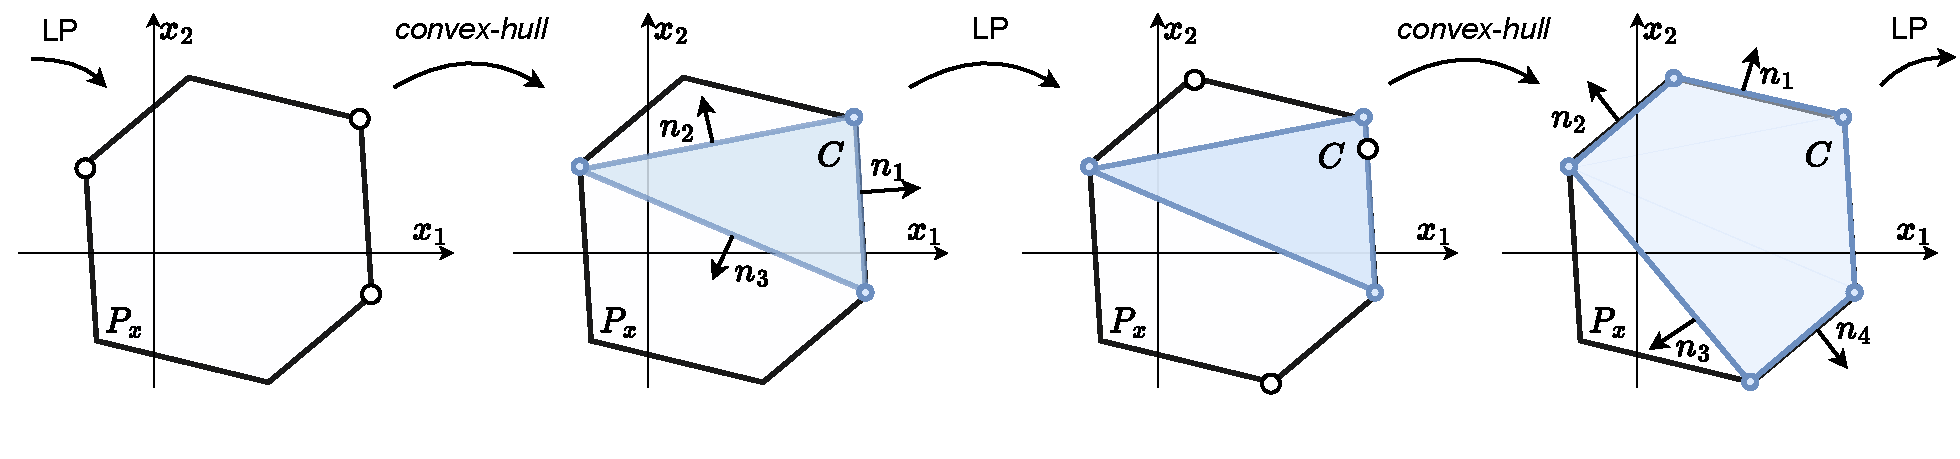
\includegraphics[width=\linewidth]{Chapters/imgs/ray_shooting.pdf}
    \caption{This figure shows the procedure of successive approximation of the polytope $\mathcal{P}_x$ using the CHM algorithm. The face normal vectors $\bm{n}_i$ of the convex-hull $\mathcal{C}$ are used with LP (\ref{eq:lin_prog}) to find new vertices which are then used to update the convex-hull $\mathcal{C}$ and furthermore improve the approximation of the polytope.}
    \label{fig:rsm}
\end{figure}

Exact vertex and facet enumeration methods, such as DDM\cite{fukuda_dd}, PIM\cite{avis_pivoting_nodate}, HPSM\cite{hyper_psm}, FME\cite{dantzig1973fourier} and similar, rely on different versions of exhaustive search in the $n$-dimensional input space, which is often much higher dimensional than the output space $n>m$. Their execution time is exponentially related to the number of vertices and the faces of the input space bounds $\mathcal{I}$\cite{avis_comparative_2015}, which can make them not practical for interactive in-the-loop applications. 

As the polytope based physical ability metrics $\mathcal{P}_x$ are usually defined in the lower-dimensional output space $\bm{x}\in \mathbb{R}^m$, several methods have been proposed performing the search in the $m$-dimensional output space. These methods are \textit{output sensitive}, having the execution time proportional to the number of vertices and the faces of the output space polytope $\mathcal{P}_x$ rather than on the input space polytope $\mathcal{I}$. 
In addition to searching in the lower dimensional output space these methods enable finding an efficient inner (or outer) approximation of the polytope $\mathcal{P}_x$, while satisfying the desired approximation accuracy. Finally, these methods evaluate the vertices and faces of the polytope $\mathcal{P}_x$ at the same time providing both $\repr{V}$ and $\repr{H}$-representation.

These methods, often called Ray Shooting Methods (RSM) or Convex-Hull Methods (CHM), first introduced by Lassez et al. \cite{lassez1992quantifier, Huynh2005PracticalIO}, iteratively approximate the polytope $\mathcal{P}_x$,  augmenting the approximation accuracy in each iteration. Their execution consists in two phases. In the first phase an initial approximation of the polytope $\mathcal{P}_x$ is constructed finding a subset of $m+1$ vertices forming an initial $m$-dimensional convex-hull $\mathcal{C}$ approximation of the polytope $\mathcal{P}_x$. In the second phase, the convex-hull approximation $\mathcal{C}$ is refined iteratively until the desired accuracy is reached. The CHM algorithms use a sequence of linear programs (LP) to find new vertices of the polytope (shooting rays) in each iteration, followed by the convex-hull algorithm to group them to the faces. An example of the CHM algorithm iterations in for $m=2$ output space is shown on Figure \ref{fig:rsm}.   

CHM algorithms have several limitations though. The resolution of the CHM algorithms relies on iterative application of the convex-hull algorithm which complexity grows exponentially for $m \geq 4$ \cite{Barber1996}. As a result, the applications of these methods have so far been limited to the low-dimensional output spaces $m\leq3$. Additionally, as different polytope formulations require different LP formulations, the implementations of these methods are often somewhat specific to their respective applications. 

There are several examples in the literature where the CHM based methods were used for improving the efficiency of different computationally expensive polytope evaluation problems. Bretl et al. \cite{Bretl2008} have proposed a CHM based algorithm for 2d ($m\!=\!2$) support region approximation for legged robot locomotion, their work has recently been extended by Audren et al. \cite{Herve2018} to the case of 3d ($m\!=\!3$) robust stability region calculation. Carmicahel et al. \cite{carmichael2011Towards, carmichael_estimating_2013} have used a simplified CHM algorithm for the calculation of the 2d ($m\!=\!2$) force capacity polytope of the human arm, based on its musculoskeletal model. Ponce and Faverjon \cite{Ponce1995} have introduced a derivative of the CHM algorithm to calculate the 2d, 2d and 4d ($m\!=\!2,3,4$) stable grasp regions for the force-closure grasp using three fingers. 

Therefore, CHM based algorithms are a promising tool for reducing complexity and improving efficiency of the polytope evaluation when the dimension $n$ of the input space is high (and/or input space limits $\mathcal{I}$ have a complex geometry) while the dimension of the output space $m$ is reasonably low $m\leq3$.


\section{Performing operations over polytopes}
\label{ch:operations_over_poly_stategies}

Once the polytopes are transformed in standard forms such as $\repr{H}$ or $\repr{V}$-representations, they can be exploited to efficiently calculate different operations over multiple polytopes, such as Minkowski sums  and intersections.

\subsection{Minkowski sum of polytopes}
\begin{figure}[!h]
    \centering
    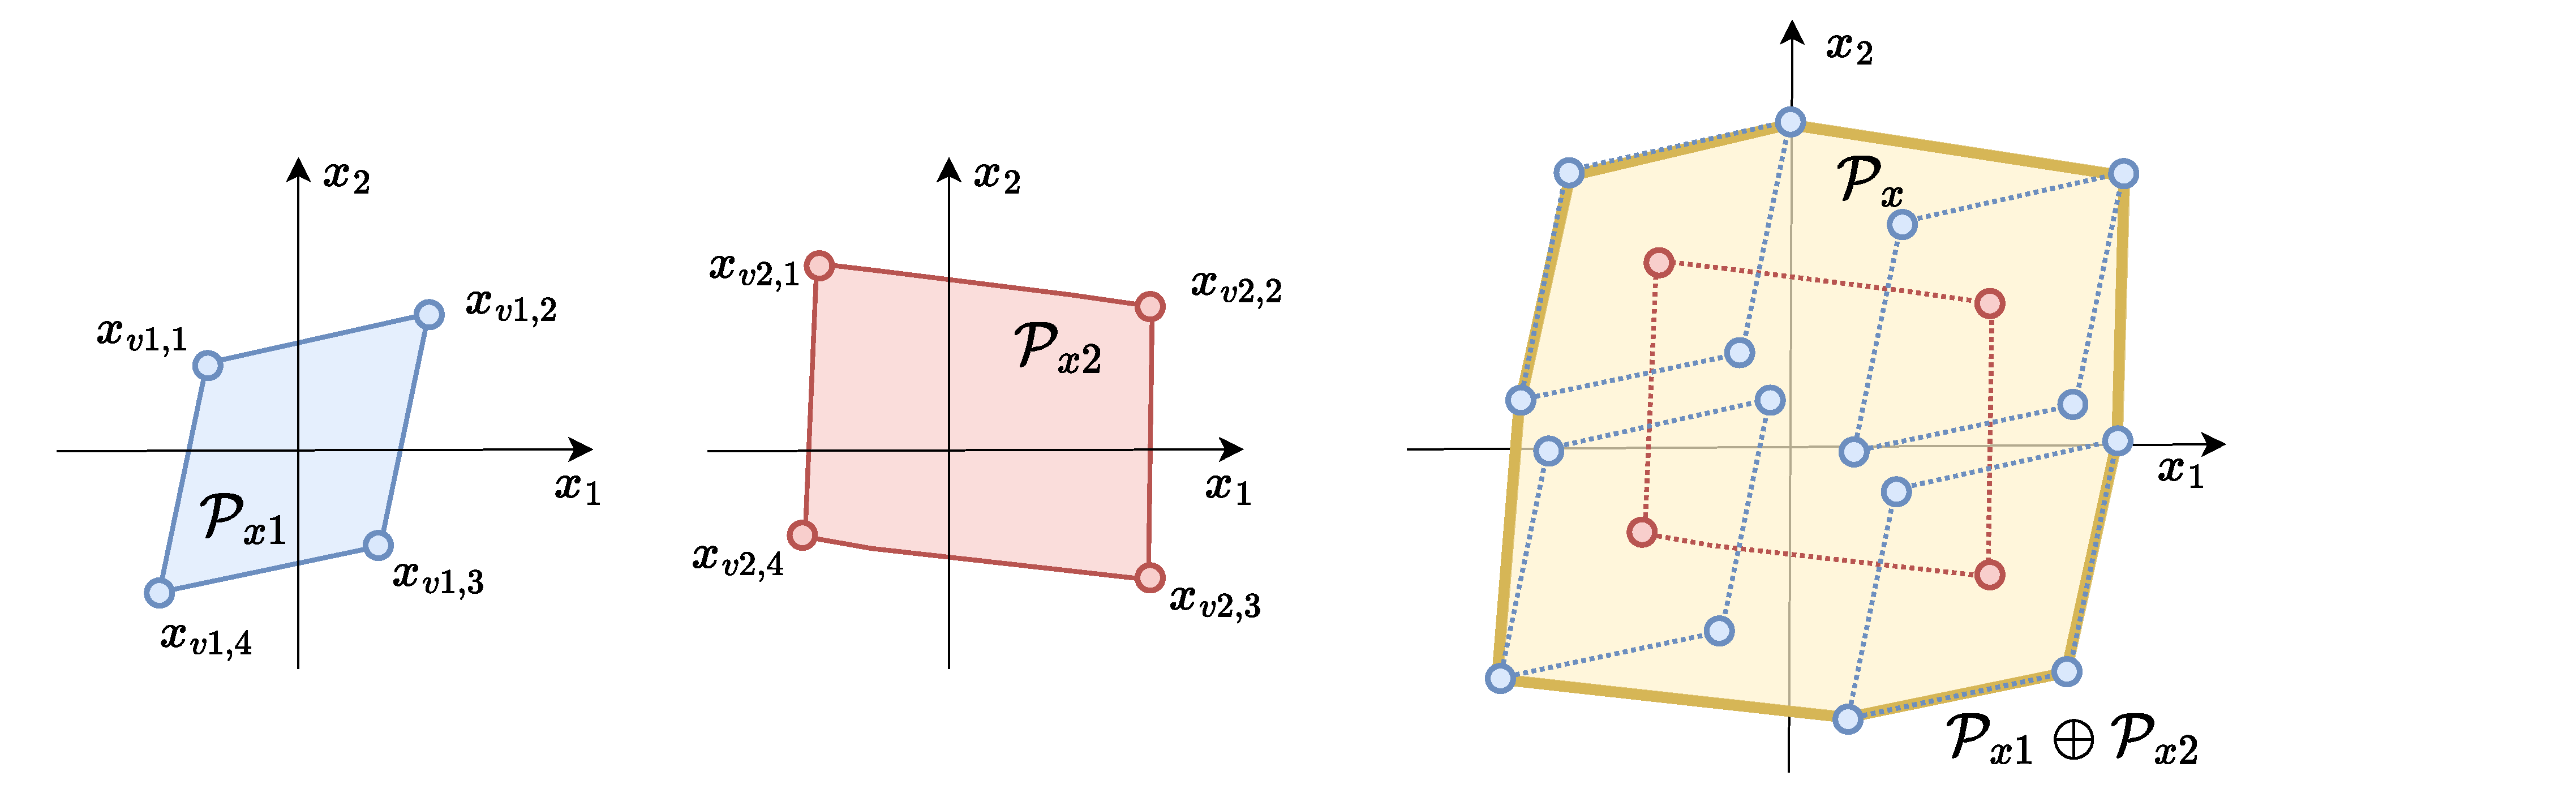
\includegraphics[width=0.9\linewidth]{Chapters/imgs/polytope_minkowski_sum.pdf}
    \caption{A 2d ($m\!=\!2$) example of the construction of the intersection of two polytopes using their $\repr{V}$-representation. The points representing the vertices of the polytope $\mathcal{P}_{x1}$ are shown in blue, and for polytope $\mathcal{P}_{x2}$ in red. The Minkowski sum polytope $\mathcal{P}_x$ is formed by calculating all the combinations of all the vertices of both polytopes, and then calculating their convex hull, the hull is shown in yellow color.}
    \label{fig:collab_sum_solution}
\end{figure}

In order to calculate Minkowski sum of multiple polytopes, for example two polytopes $\mathcal{P}_{x1}$ and $ \mathcal{P}_{x2}$
\begin{equation}
    \mathcal{P}_x = \mathcal{P}_{x1} \oplus \mathcal{P}_{x2}
\end{equation}
the most straight-forward approach is to express both polytopes in their $\repr{V}$-representation form
\begin{equation}
    \mathcal{P}_{x1} = conv\{
    \bm{x}_{v1,1},~\bm{x}_{v1,2},~\ldots~,\bm{x}_{v1,N_1}\}
\end{equation}
\begin{equation}
    \mathcal{P}_{x2} =  conv\{\bm{x}_{v2,1},~\bm{x}_{v2, 2},~\ldots~,\bm{x}_{v2,N_2}\}
\end{equation}
where polytope $\mathcal{P}_{x1}$ has $N_1$ vertices $\bm{x}_{v1,i}\in \mathbb{R}^m$, and polytope $\mathcal{P}_{x2}$ has $N_2$ vertices $\bm{x}_{v2,i}\in \mathbb{R}^m$.

Then the Minkowski sum of the polytopes can be found as the convex-hull of all the $N_1\!\cdot\!N_2$ combinations of all the vertices of the two polytopes
\begin{equation}
\begin{split}
    \mathcal{P}_x =  conv\big\{&\bm{x}_{v1,1} + \bm{x}_{v2,1},~ \ldots~,\bm{x}_{v1, N_1} + \bm{x}_{v2,1},\\&\bm{x}_{v1,1} + \bm{x}_{v2,2},~\ldots~,\bm{x}_{v1, N_1} + \bm{x}_{v2,2},\\&~\ldots~\\
    &\bm{x}_{v1, 1}  +\bm{x}_{v2,N_2}, ~\ldots~ ,\bm{x}_{v1, N_1} +\bm{x}_{v2,N_2}\big\}
\end{split}
\end{equation}
These $N_1\!\cdot\!N_2$ are not all vertices of the polytope $\mathcal{P}_x$, some of them are inside of the polytope, as shown on a graphical example of the Minkowski sum of two  2d ($m=2$) polytopes on Figure \ref{fig:collab_sum_solution}. In order to find the minimal set of vertices of the polytope $\mathcal
{P}_x$, defining its $\repr{V}$-representation, different convex-hull algorithms \cite{Barber1996} can be used.

Once the $\repr{V}$-representation is determined, different standard facet enumeration algorithms, such as DDM\cite{fukuda_dd} or PIM\cite{avis_pivoting_nodate}, can be used to efficiently find its $\repr{H}$-representation.


\paragraph*{Special case - projection formulation}
A special case of simplified Minkowski sum calculation arises when polytopes $\mathcal{P}_{x1}$ and $\mathcal{P}_{x2}$ both have projection formulation
\begin{equation}
    \mathcal{P}_{x1}=\{\bm{x}_1\in\mathbb{R}^m |~ \bm{x}_1 = B_1\bm{y}_1,~\bm{y}_1 \in \mathcal{I}_1  \}
\end{equation}
\begin{equation}
    \mathcal{P}_{x2}=\{\bm{x}_2\in\mathbb{R}^m |~ \bm{x}_2 = B_2\bm{y}_2,~\bm{y}_2 \in \mathcal{I}_2  \}
\end{equation}
where both polytopes are defined in the comon $m$ dimensional output space $\bm{x}_1,\bm{x}_2\in\mathbb{R}^m$, while their input spaces $\bm{y}_1\in\mathbb{R}^{n_1}$,$\bm{y}_2\in\mathbb{R}^{n_2}$ might have different dimensions $n_1\neq n_2$ and are limited, in generic case, by polytope input sets $\mathcal{I}_1$ and $\mathcal{I}_2$.
\begin{equation}
    \mathcal{I}_{1}=\{\bm{y}_1\in\mathbb{R}^{n_1} ~|~ H_1\bm{y}_1 \leq \bm{d}_1\}, \qquad
    \mathcal{I}_{2}=\{\bm{y}_2\in\mathbb{R}^{n_2} ~|~ H_2\bm{y}_2 \leq \bm{d}_2\}
\end{equation}

As the Minkowski sum of two polytopes can then be expressed as the achievable set of output variable $\bm{x}\in\mathbb{R}^m$ corresponding the sum of the variables $\bm{x}_1$ and $\bm{x}_2$
\begin{equation}
    \mathcal{P}_{x}= \mathcal{P}_{x1} \oplus \mathcal{P}_{x2} = \{\bm{x}\in\mathbb{R}^m ~|~ \bm{x} =  \bm{x}_1 + \bm{x}_2, \quad \bm{x}_1 \in \mathcal{P}_{x1}, ~\bm{x}_2 \in \mathcal{P}_{x2},  \}
\end{equation}
the projection formulation of their Minkowski sum can be expressed directly
\begin{equation}
    \mathcal{P}_{x}=\left\{\bm{x}\in\mathbb{R}^m ~\bigg|~ 
    \bm{x} = \begin{bmatrix}
        B_1 & 0 \\
        0 & B_2
    \end{bmatrix}\begin{bmatrix}
        \bm{y}_1 \\
        \bm{y}_2
    \end{bmatrix}, ~\begin{bmatrix}
        H_1  \\
        H_2
    \end{bmatrix} \begin{bmatrix}
        \bm{y}_1 \\
        \bm{y}_2
    \end{bmatrix} \leq \begin{bmatrix}
        \bm{d}_1  \\
        \bm{d}_2
    \end{bmatrix} \right\}
\end{equation}

Finding the $\repr{V}$ and $\repr{H}$-representation of this polytope can then be done using the approaches  for polytope with projection formulation, described in chapter \ref{ch:projection_algos}.

\paragraph*{} The same logic can be used if the Minkowski sum is calculated for more than two polytopes 
\begin{equation}
    \mathcal{P}_x = \mathcal{P}_{x1} \oplus \mathcal{P}_{x2} \oplus ~\cdots
\end{equation}

\subsection{Polytope intersection}

\begin{figure}[!h]
    \centering
    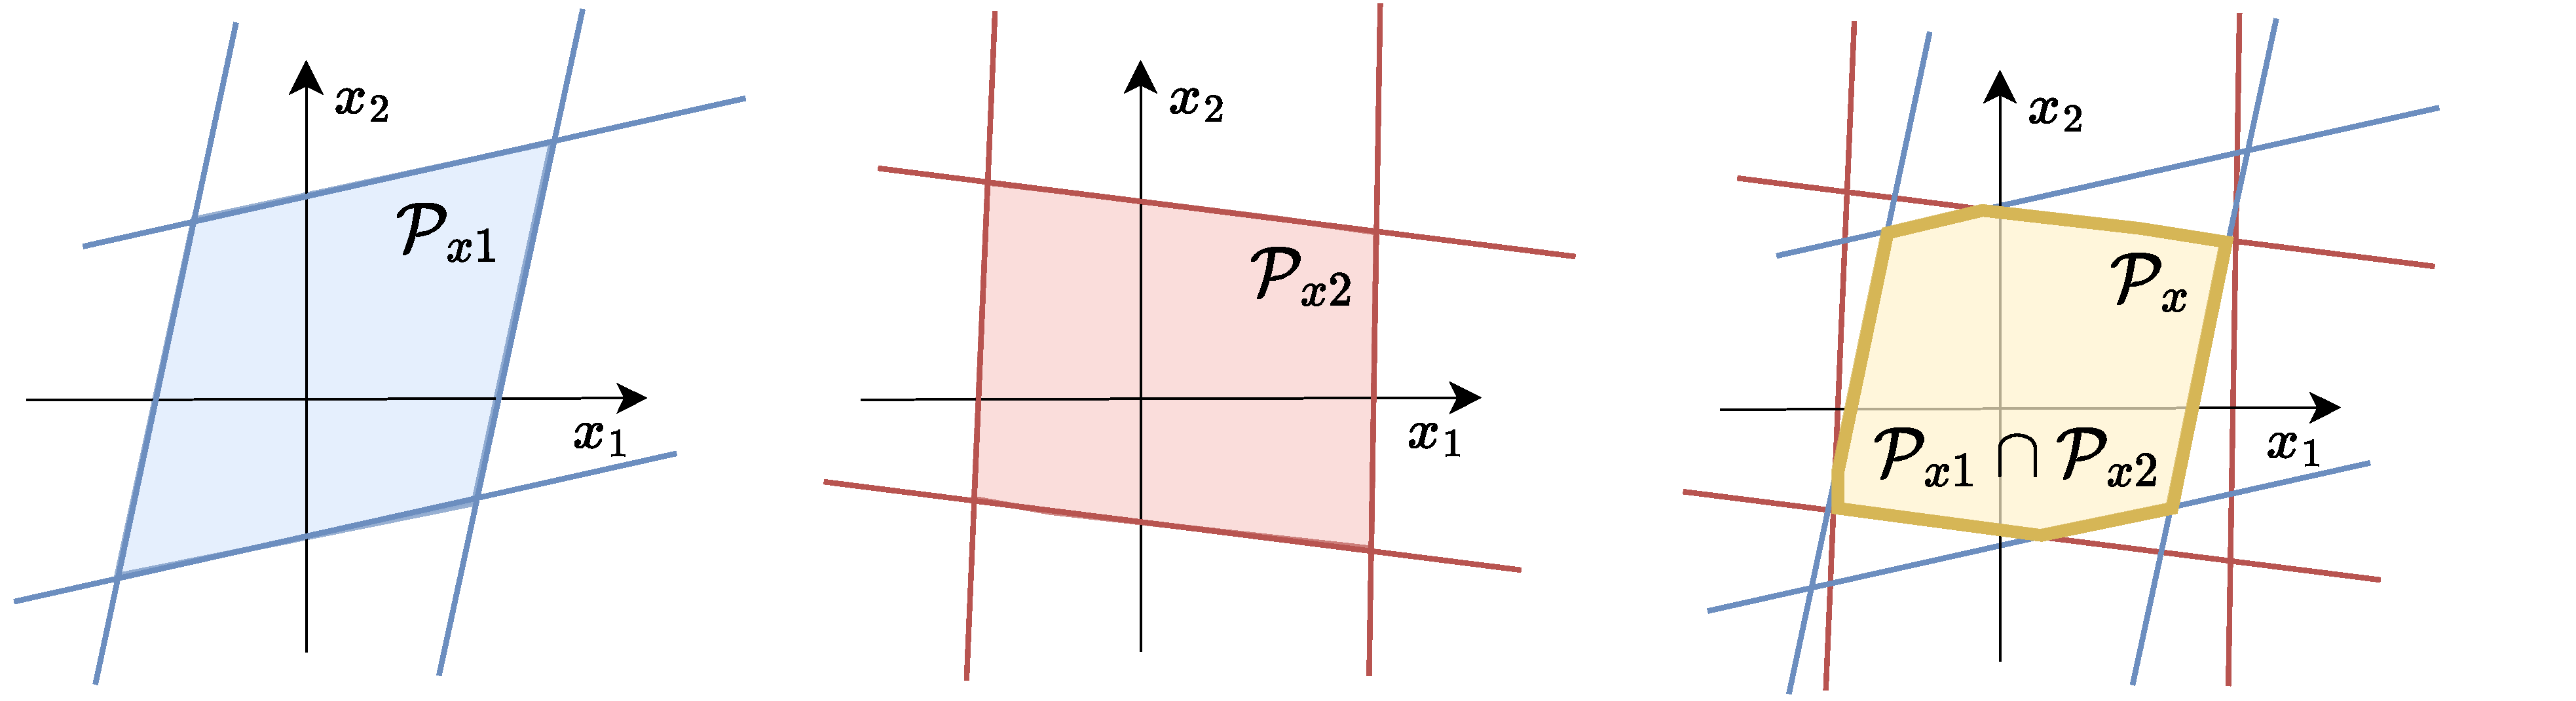
\includegraphics[width=0.8\linewidth]{Chapters/imgs/polytope_intersection.pdf}
    \caption{A 2d ($m\!=\!2$) example of the construction of the intersection of two polytopes using their $\repr{H}$-representation. The lines representing half-planes of the polytope $\mathcal{P}_{x1}$ are shown in blue, and for polytope $\mathcal{P}_{x2}$ in red. The intersection polytope $\mathcal{P}_x$ is formed by including all of their half-planes, where the space representing their intersection is shown in yellow.}
    \label{fig:collab_intesection_solution}
\end{figure}

In order to calculate an intersection of multiple polytopes, for example two polytopes $\mathcal{P}_{x1}$ and $ \mathcal{P}_{x2}$
\begin{equation}
    \mathcal{P}_x = \mathcal{P}_{x1} \cap \mathcal{P}_{x2}
\end{equation}
the simplest approach is to transform both polytopes to their $\repr{H}$-representation
\begin{equation}
    \mathcal{P}_{x1} = \{\bm{x}\in\mathbb{R}^m ~|~ H_1\bm{x}\leq \bm{d}_1\}
\end{equation}
\begin{equation}
    \mathcal{P}_{x2} = \{\bm{x}\in\mathbb{R}^m ~|~ H_2\bm{x}\leq \bm{d}_2\}
\end{equation}
where polytopes $\mathcal{P}_{x1}$ and  $\mathcal{P}_{x2}$ represent limits of the same output variable $\bm{x}\in\mathbb{R}^m$. Additionally matrices $H_i\in\mathbb{R}^{m\times N_i}$ and vectors $\bm{d}_i\in\mathbb{R}^{N_i}$ define the half-plane representation of the polytopes $\mathcal{P}_{xi}$ with $N_i$ faces.

Given their $\repr{H}$-representations the intersections of these polytopes can be expressed directly as
\begin{equation}
    \mathcal{P}_x = \left\{\bm{x}\in\mathbb{R}^m ~\bigg|~ \begin{bmatrix}
        H_1\\
        H_2
    \end{bmatrix}\bm{x}\leq \begin{bmatrix}
        \bm{d}_1\\
        \bm{d}_2
    \end{bmatrix}\right\}
\end{equation}
by stacking their matrices $H_i$ and vectors $\bm{d}_i$ forming the $\repr{H}$-representation of the polytope $\mathcal{P}_x$. The obtained $\repr{H}$-representation might not be minimal though, it might have some redundant inequalities. If the application requires it, they can be removed using standard algorithms \cite{Paulraj2006}.
A visual example of constructing the intersection of $m=2$ dimensional polytopes using their $\repr{H}$-representation is shown on Figure \ref{fig:collab_intesection_solution}.

Once the $\repr{H}$-representation is determined, different standard vertex enumeration algorithms, such as DDM\cite{fukuda_dd} or PIM\cite{avis_pivoting_nodate}, can be used to find its $\repr{V}$-representation.

\paragraph*{Special case - intersection formulation}

A special case of simplified polytope intersection calculation arises when polytopes $\mathcal{P}_{x1}$ and $\mathcal{P}_{x2}$ both have intersection formulation
\begin{equation}
    \mathcal{P}_{x1}=\{\bm{x}\in\mathbb{R}^m |~ A_1\bm{x} = \bm{y}_1,~\bm{y}_1 \in \mathcal{I}_1  \}
\end{equation}
\begin{equation}
    \mathcal{P}_{x2}=\{\bm{x}\in\mathbb{R}^m |~ A_2\bm{x} = \bm{y}_2,~\bm{y}_2 \in \mathcal{I}_2  \}
\end{equation}
where both polytopes are defined in the common $m$ dimensional output space $\bm{x}\in\mathbb{R}^m$, while their input spaces $\bm{y}_1\in\mathbb{R}^{n_1}$,$\bm{y}_2\in\mathbb{R}^{n_2}$ might have different dimensions $n_1\neq n_2$ and are limited, in generic case, by polytope input sets $\mathcal{I}_1$ and $\mathcal{I}_2$.
\begin{equation}
    \mathcal{I}_{1}=\{\bm{y}_1\in\mathbb{R}^{n_1} ~|~ H_1\bm{y}_1 \leq \bm{d}_1\}, \qquad
    \mathcal{I}_{2}=\{\bm{y}_2\in\mathbb{R}^{n_2} ~|~ H_2\bm{y}_2 \leq \bm{d}_2\}
\end{equation}

Using these polytope formulations their intersection polytope can be expressed in the intersection formulation by stacking the equations
\begin{equation}
    \mathcal{P}_{x}=\left\{\bm{x}\in\mathbb{R}^m ~\bigg|~ 
   \begin{bmatrix}
        A_1 \\
        A_2
    \end{bmatrix} \bm{x} = \begin{bmatrix}
        \bm{y}_1 \\
        \bm{y}_2
    \end{bmatrix}, ~\begin{bmatrix}
        H_1  \\
        H_2
    \end{bmatrix} \begin{bmatrix}
        \bm{y}_1 \\
        \bm{y}_2
    \end{bmatrix} \leq \begin{bmatrix}
        \bm{d}_1  \\
        \bm{d}_2
    \end{bmatrix} \right\}
\end{equation}


Finding the $\repr{V}$ and $\repr{H}$-representation of this polytope can then be done using the approaches for polytope with intersection formulation, described in chapter \ref{ch:intersection_algos}.


\paragraph*{} The same logic can be used if the intersection is calculated for more than two polytopes 
\begin{equation}
    \mathcal{P}_x = \mathcal{P}_{x1} \cap \mathcal{P}_{x2} \cap ~\cdots
\end{equation}

% \subsection{Convex hulls of polytopes}
% \begin{figure}[!h]
%     \centering
%     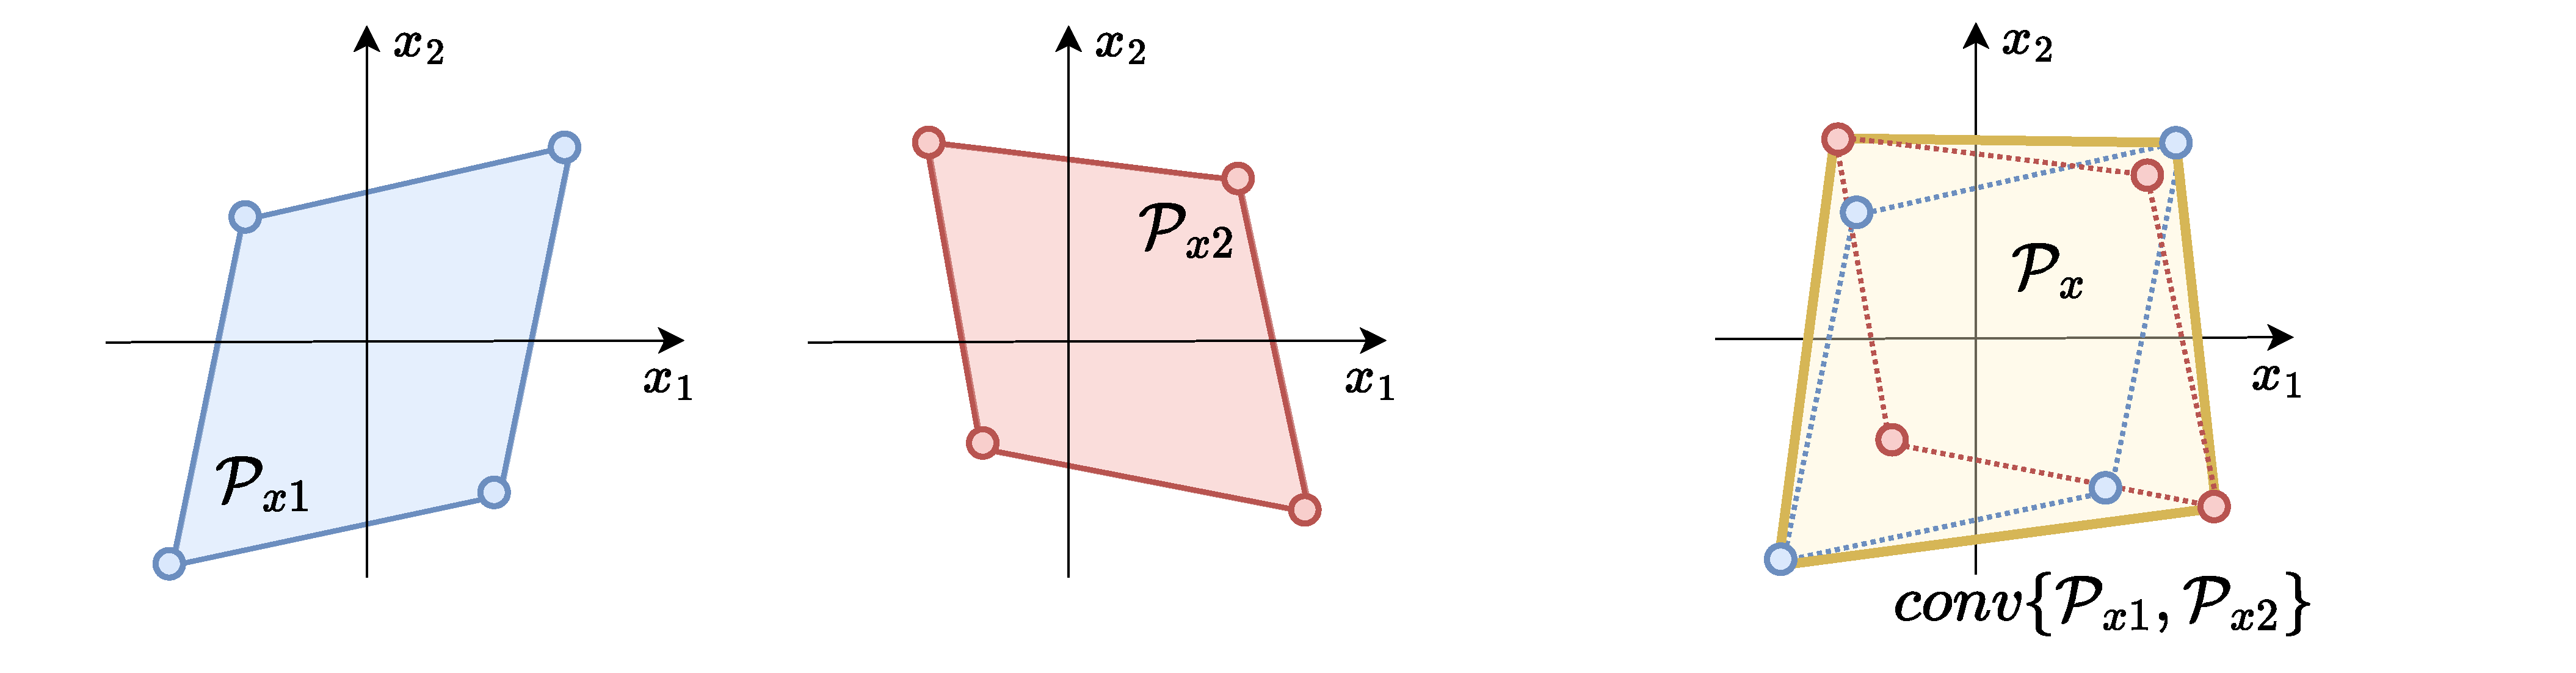
\includegraphics[width=0.8\linewidth]{Chapters/imgs/polytope_union.pdf}
%     \caption{Caption}
%     \label{fig:collab_union_solution}
% \end{figure}

% \begin{equation}
%     \mathcal{P}_x = \mathcal{P}_{x1} \cup \mathcal{P}_{x2}
% \end{equation}

% \begin{equation}
%     \mathcal{P}_{x1} = conv\{\bm{x}_{v1,1},~\bm{x}_{v1,2},~\ldots~,\bm{x}_{v1,N_1}\}
% \end{equation}
% \begin{equation}
%     \mathcal{P}_{x2} =  conv\{\bm{x}_{v2,1},~\bm{x}_{v2, 2},~\ldots~,\bm{x}_{v2,N_2}\}
% \end{equation}

% \begin{equation}
% \begin{split}
%     \mathcal{P}_x =  conv\big\{&\bm{x}_{v1,1},~\bm{x}_{v1,2},~\ldots~,\bm{x}_{v1,N_1},\\
%     &\bm{x}_{v2,1},~\bm{x}_{v2, 2},~\ldots~,\bm{x}_{v2,N_2}\big\}
% \end{split}
% \end{equation}


\section{Conclusion}

% The aim of this chapter is to provide a set of tools for efficiently transforming polytopes of physical abilities of humans and robots into more standard forms suitable for practical applications. 

% This chapter is focused on two most used polytope representations are called vertex or $\repr{V}$ and half-plane or $\repr{H}$-representation. These representations enable using the polytopes with different visualisation tools, as triangulated meshes, and with different optimisation based applications, such as robot control or trajectory planning. Additionally, these representations enable performing efficient operations over multiple polytopes such as Minkowski sums and intersections. 

% Many well known algorithms are proposed in the literature, capable of transforming different polytope formulations in their $\repr{H}$ or $\repr{V}$-representation. However, they are usually defined for very specific set of polytope formulations.  Therefore, this chapter brings the classification of physical abilities of humans and robots with respect to their polytope formulation and gives an overview of applicable techniques for transforming them to their $\repr{H}$ or $\repr{V}$-representation. Additionally, the chapter demonstrates the use of the standard representations to efficiently calculate Minkowski sum and intersection operations over multiple polytopes, and discusses several special cases based on the polytope formulation.

% Even though this chapter provides a set of tools for transforming (vertex and facet enumeration) all the generic families of polytopes present when characterising physical abilities of humans and robots, finding an appropriate algorithm for a given application, in terms of time-efficiency, is not always straight-forward especially if it requires online (real-time) execution. 
% Polytope enumeration strategies are relatively computationally expensive algorithms. Their complexity depends on many different factors, such as polytope formulation, the dimensions of input and output space, the complexity of the polytope (number of faces and vertices) and similar. 
% Therefore, in many cases the algorithms that perform the best are the ones that are developed specifically for their respective applications, often exploiting their specific problem formulation and geometry.


% However, being able to represent the physical abilities of humans and robots using the standard polytope representations opens many doors for their potential applications, especially in the context of human robot interaction. Visualising an accurate representation of robot's physical abilities to the operator, might help to enhance the human's understanding about robot's current state and provide a detailed insight about its abilities. On the other hand, as polytopes can be easily integrated in different optimisation problems, they might enable creating more human-centred robot control or trajectory planning strategies which could take in consideration both human's and robot's physical abilities at the same time.



In conclusion, this chapter aimed to provide a set of tools for efficiently transforming polytopes representing the physical abilities of humans and robots into more standardised forms suitable for practical applications. The focus was put on the two widely used polytope representations: vertex or $\repr{V}$ and half-plane or $\repr{H}$-representations. These representations offer various advantages, including compatibility with visualisation tools, in a for triangulated meshes, and optimisation-based applications like robot control and trajectory planning. Additionally, they enable efficient operations like Minkowski sums and intersections over multiple polytopes.

While the literature presents numerous algorithms for transforming polytope formulations into their $\repr{H}$ or $\repr{V}$-representation, these algorithms are often tailored to specific sets of polytope formulations. Hence, this chapter classified the physical abilities of humans and robots based on their polytope formulation and provided an overview of applicable techniques for transforming them into their $\repr{V}$ or $\repr{V}$-representation. Furthermore, it demonstrated the practical utilisation of standard representations for efficient calculation of Minkowski sum and intersection operations, while also discussing several special cases based on polytope formulation.

It is worth noting that despite providing tools for transforming all generic families of polytopes, finding the most suitable algorithm for a given application in terms of time-efficiency can be challenging, especially when real-time execution is required. Polytope enumeration strategies are computationally expensive, and their complexity depends on various factors such as polytope formulation, input and output space dimensions, and polytope complexity (e.g., number of faces and vertices). Consequently, algorithms specifically developed for respective applications, leveraging their problem formulation and geometry, often perform the best.

Nevertheless, representing the physical abilities of humans and robots using standard polytope representations opens up numerous possibilities for their potential applications, particularly in the context of human-robot interaction. Accurately visualising a robot's physical abilities to the operator has a potential to enhance human understanding of the robot's current state and provide detailed insight into its capabilities. Moreover, integrating polytopes into different optimisation problems enables the creation of more human-centred robot control or trajectory planning strategies that consider both human and robot physical abilities simultaneously.

In summary, this chapter brings an overview of generic polytope formulations and their transformation techniques for physical abilities of humans and robots. While challenges exist in algorithm selection and computational efficiency, the use of standardised representations might enable their use with a wide range of applications, having a potential to enhance human-robot interaction and enable more human-centred control and motion planning strategies.